\chapter{机械振动和机械波}
前面我们已经学过:在平衡力作用下的匀速运动,在大小和方向都不变的恒力作用下的匀变速运动,在大小不变而方向改变的向心力作用下的匀速圆周运动.现在我们要学习在大小和方向都改变的力作用下的机械振动,以及机械振动的传播形成的机械波.

到电学、光学部分将学习的交流电、电磁振荡、电磁波、光波,跟机械振动、机械波相比,虽然物理本质不同,有许多特征和规律却是相同的,因此,机械振动和机械波的知识,对于学习电学、光学、电工学和无线电工学等等也很重要.

这一章的内容较多,我们分三部分学习.第一部分是机械振动,第二部分是机械波,第三部分是声学初步知识.
\section{机械振动}
\subsection{机械振动}
\subsubsection{产生振动的条件}

物体(或者物体的一部分)在平衡位置附近来回做往复运动,叫做\textbf{机械振动},常常简称为振动.挂在弹簧下端的重物的上下振动(图9.1),单摆的小球的左右摆动,是振动的典型例子.

把挂在弹簧下端的重物从平衡位置$O$拉下再放开,它就从最低点$B$向着平衡位置$O$运动并越过$O$运动到最高点$C$,然后再向着平衡位置$O$运动并越过$O$回到最低点$B$.以后重物在平衡位置附近经过多次重复的上下振动,最后停在平衡位置,把单摆的小球拉开再放手,小球就在平衡位置附近左右振动,经过多次重复,最后停在平衡位置.击一下鼓或敲一下锣,鼓膜或锣面就在平衡位置附近做起伏振动,经过多次重复,最后停在平衡位置.

为什么物体会做这样的运动呢?从地面竖直上抛的物体能返回地面,是因为受到指向地面的力的作用.与此类似,物体所以能在平衡位置附近做往复运动而不远离,并经多次重复以后还停在平衡位置,是因为受到指向平衡位置的力的作用,使振动物体回到平衡位置的力叫做\textbf{回复力}.

\textbf{每当物体离开平衡位置就会受到回复力的作用,这是产
    生振动的第一个必要条件},应该注意,回复力也是根据力的效果命名的,它可能是弹力,可能是重力,还可能是它们的合力或分力,后面将讲到回复力的实例.

同一个单摆,在空气里,由于阻力很小,衰减很慢,可以重复摆动许多次才停下.在水里,阻力相当大,衰减很快,摆不了几次就停下,在很粘的油里,阻力很大,离开平衡位置的摆球虽然还能缓慢地回到平衡位置,但是到达平衡位置时的速度
实际等于零,所以不会产生振动,可见,\textbf{产生振动的第二个必要条件是阻力足够小}.

\subsubsection{表征振动的物理量}

研究匀速和变速直线运动的时候,解决的问题主要是确定物体在任一时刻的位置和速度.研究振动,同样需要确定物体在任一时刻的位置和速度,这是二者相同的地方.因此,研究振动也需要位移、速度、加速度等物理量,但是振动有它自己的特点,需要引入新的物理量来表示这种特点,至于怎样确定振动物体在任一时刻的位置和速度,因为计算比较复杂,本书就不讲了.

振动是一种往复运动,振动物体的位移不象匀速或变速直线运动那样可以继续增大下去,而是有一个最大位移,否则就不成其为振动了.振动物体离开平衡位置的最大距离叫做\textbf{振幅}.图9.1中振动的振幅就等于$OB$或$OC$.振幅是表示振动幅度的大小或振动强弱的物理量.

\begin{figure}[H]\centering
    \begin{tikzpicture}[>=stealth,scale=1.2]
        \tikzstyle{spring1}=[decorate,decoration={aspect=0.5, segment length=4mm, amplitude=3mm,zigzag}]
        \tikzstyle{spring2}=[decorate,decoration={aspect=0.5, segment length=3mm, amplitude=3mm,zigzag}]
        \tikzstyle{spring3}=[decorate,decoration={aspect=0.5, segment length=2mm, amplitude=3mm,zigzag}]
        \fill [pattern = north east lines] (-4,0) rectangle (-2,.25);
        \fill [pattern = north east lines] (-1,0) rectangle (1,.25);
        \fill [pattern = north east lines] (2,0) rectangle (4,.25);
        \draw(-4,0)--(-2,0);  \draw(-1,0)--(1,0);  \draw(2,0)--(4,0);
        \draw [fill=gray!30] (-3.5, -4.3) rectangle (-2.5, -4);
        \draw [fill=gray!30] (-.5, -5.3) rectangle (.5, -5);
        \draw [fill=gray!30] (2.5, -3.3) rectangle (3.5, -3);
        \draw [spring2](-3,0)--(-3,-4);
        \draw [spring1](0,0)--(0,-5);
        \draw [spring3](3,0)--(3,-3);
        \draw [dashed](-2, -3)node[left]{$C$}--(2.25,-3);
        \draw [dashed](-2, -4)node[left]{$O$}--(-.25,-4);
        \draw [dashed](-2, -5)node[left]{$B$}--(-.25,-5);
        \draw [<->](-1.5, -3)--node[fill=white]{$A$}(-1.5,-4);
        \draw [<->](-1.5, -5)--node[fill=white]{$A$}(-1.5,-4);
        \draw [->] (-3.75, -4.25)--(-3.75, -3.75);
        \draw [<-] (-4, -4.25)--(-4, -3.75);
    \end{tikzpicture}
    \caption{弹簧下端的重物的上下振动}
\end{figure}


振动的最大特点是重复性,或者说周期性,所谓周期性,就是振动物体的位移和速度经过一定时间之后又重复地回到原来的数值.例如在图9.1中,振动物体由$B$点经过$O$到达$C$点,再经过$O$回到$B$点,即完成一次全振动,位移和速度就
重复地回到原来的数值,完成一次全振动经过的时间叫做\textbf{周期},周期是表示振动快慢的物理量.

振动的快慢也可以用频率来表示,在1秒内完成全振动的次数叫做\textbf{频率},频率的单位是\textbf{赫兹},简称赫,国际符号是
Hz,1秒钟振动1次就是1赫.1秒钟振动$n$次就是$n$赫.

如果用$T$(秒)表示周期,用$f$(赫)表示频率,那么
\[f=\frac{1}{T},\qquad T=\frac{1}{f}\]

振幅、周期或频率是表征整个振动的物理量.一个振动,如果知道了它的振幅、周期或频率,我们就从整体上把握了振动的情况.

\subsection*{练习一}
\begin{enumerate}
    \item 设图9.1中振幅是2厘米,完成一次全振动,振动物体通过的路程是多少厘米?如果频率是5赫,振动物体每秒通过的路程是多少厘米?
    \item 设图9.1中振幅是2厘米,取竖直向上的方向作为正方向,物体运动到点$C$时对平衡位置的位移是多大?运动到点$B$时对平衡位置的位移又是多大?
\end{enumerate}


\subsection{简谐振动}
振动现象是很普遍的,是多种多样的,我们怎样着手研究它呢?小鸟从树枝上飞开,树枝就振动起来,这个现象看来比较简单,可是真要研究它,所要考虑的因素却很复杂,不便于我们着手研究.跟研究其他现象一样,研究振动现象也
要从最简单、最基本的振动来着手.前一节我们说过,产生振动的第一个必要条件是要有回复力的作用.回复力的性质是各种各样的,我们希望着手被研究的那种振动,所受的回复力要比较简单.假如回复力是弹簧的弹力,我们希望弹簧的形变在弹性限度之内,因为这时弹力跟形变成正比.产生振动的第二个必要条件是阻力足够小.既然如此,我们着手研究的时候,暂时就不去考虑阻力,而研究一种无阻力的理想化的振动,这就是这一节要讲的简谐振动.

这里我们再一次遇到所谓理想化的方法.这是研究物理现象经常采用的方法,这样做的好处是使复杂问题变得简单,便于人们就这种简单情况深入探讨,然后再把暂时被抛开的因素和其他因素考虑进去,逐步由简单到复杂,简谐振动不但是研究复杂振动的基础,它本身也具有实际意义,许多复杂的振动在振幅小的情况下可以近似地看作是简谐振动,一切复杂的振动都可以看作是若干振幅、频率不同的简谐振动合成的.

简谐振动的特点是什么呢?下面我们通过一个典型例子来说明,这个典型例子就是弹簧振子.

\subsubsection{弹簧振子}

\begin{figure}[H]\centering
    \begin{tikzpicture}[>=stealth,thick,scale=1.3]
        \tikzstyle{spring1}=[decorate,decoration={aspect=0.5, segment length=4mm, amplitude=3mm,coil}]
        \tikzstyle{spring2}=[decorate,decoration={aspect=0.5, segment length=3mm, amplitude=3mm,coil}]
        \tikzstyle{spring3}=[decorate,decoration={aspect=0.5, segment length=2mm, amplitude=3mm,coil}]
        \fill [pattern = north east lines] (-.25,2) rectangle (0,3);
        \fill [pattern = north east lines] (6,2) rectangle (6.25,3);
        \fill [pattern = north east lines] (-.25,0) rectangle (0,1);
        \fill [pattern = north east lines] (6,0) rectangle (6.25,1);
        \fill [pattern = north east lines] (-.25,-1) rectangle (0,-2);
        \fill [pattern = north east lines] (6,-1) rectangle (6.25,-2);
        \draw(0,2)--(0,3);  \draw(0,0)--(0,1);  \draw(0,-1)--(0,-2);
        \draw(6,2)--(6,3);  \draw(6,0)--(6,1);  \draw(6,-1)--(6,-2);
        \draw(0,2.5)--(6,2.5); \draw(0,.5)--(6,.5); \draw(0,-1.5)--(6,-1.5);
        \draw [->, ultra thick](5,.5)--(4.2,.5)node [below]{$F$};
        \draw [->, ultra thick](3,-1.5)--(3.8,-1.5)node [below]{$F$};
        \draw [dashed] (3, .5)--node [fill=white]{$C$}(3,-1.5);
        \draw [dashed] (4, .5)--node [fill=white]{$O$}(4,-1.5);
        \draw [dashed] (4, .5)--node [fill=white]{$O$}(4,2.5);
        \draw [dashed] (5, .5)--node [fill=white]{$B$}(5,-1.5);
        \draw [shade] (4, 2.5) circle(.2);
        \draw [shade] (5,.5) circle(.2);
        \draw [shade] (3,-1.5) circle(.2);
        \draw [spring2](0,2.5)--(4-.2,2.5);
        \draw [spring1](0,.5)--(5-.2,.5);
        \draw [spring3](0,-1.5)--(3-.2,-1.5);
    \end{tikzpicture}
    \caption{弹簧振子的振动}
\end{figure}

照图9.2那样,把连在一起的弹簧和小球穿在水平杆上,弹簧左端固定在支架上,小球可以在杆上滑动.杆非常光滑,小球滑动时的摩擦力可以忽略.弹簧的质量比小球的小得多,也可以忽略.这样就成了一个弹簧振子,振子静止在$O$点时,它受的重力和杆的支持力互相平衡,弹簧没有形变因而对它没有弹力作用,$O$点就是振子的平衡位置.把它拉离平衡位置再放开,它就沿水平杆左右振动.

在振子振动过程中,重力和杆的支持力总是互相平衡,对振动不起作用,对振动起作用的只是弹簧作用在振子上的弹力.振子运动到$O$点右侧时,弹簧拉长,振子对平衡位置的位移方向向右,弹簧对振子的弹力方向向左.振子运动到$O$点左侧时,弹簧压缩,振子对平衡位置的位移方向向左,弹簧对振子的弹力方向向右.可见在这个弹簧振子上,总是指向平衡位置的回复力是弹簧对振子的弹力,这个弹力的方向跟振子对平衡位置的位移方向相反.

根据胡克定律,在振幅不大(弹簧不超出弹性限度)的情况下,弹簧振子回复力$F$的大小跟弹簧伸长或缩短的长度$x$成正比,而这个长度就是振子对平衡位置的位移的大小,因此回复力$F$的大小跟这个位移$x$的大小成正比.刚刚讲过,回复力的方向跟这个位移的方向相反,这样,用下式就可以把回复力的大小和方向都表示出来:
\[F=-kx\]
式中$k$是比例常数,对于弹簧振子来说,就等于弹簧的倔强系数.式中的负号表示回复力的方向跟位移的方向相反.

这种在跟对平衡位置的位移成正比而方向相反的回复力
作用下的振动,叫做\textbf{简谐振动}.

用$m$代表振子的质量,用$a$代表振子的加速度,根据牛顿
第二定律$F=ma$ 可以得到
\[a=-\frac{k}{m}x\]

上式表明,在简谐振动中,加速度也跟位移成正比而方向相反.在图9.2里,当振子从$O$向右运动时,加速度的方向向左,并且随着位移增大而增大,即振子做变减速运动,到速度减小到零时,振子运动到右端最大位移处$B$,加速度也增大到最大值.振子从$B$向$O$运动的过程中,加速度的方向仍向左,并且随位移的减小而减小,即振子做初速度为零的变加速运动.当振子回到$O$点时,位移减小到零,加速度也减小到零,而速度增大到最大值,方向向左.由于惯性,振子就以这个速度继续向左运动,在越过$O$点以后,加速度的方向向右,
并且随位移的增大而增大,振子做变减速运动,到速度减小到零时,振子运动到左端最大位移处$C$,加速度也增大到最大值.然后振子从$C$向右运动,加速度的方向仍向右,并且随位移的减小而减小,即振子做初速度为零的变加速运动.当振子回到$O$点时,位移、加速度都减小到零,而速度增大到最大值,方向向右.此后将重复上述的过程.

值得注意的是,在简谐振动中速度与加速度的变化不一样,加速度最大时速度等于零,加速度等于零时速度最大.

\subsubsection{简谐振动的周期}

简谐振动的周期跟什么有关呢?在回复力的表示式$F=-kx$中,$k$越大,回复力越大,振子产生的加速度越大,振子来回振动得越快,因而周期越短.在图9.2中用不同倔强系数的弹簧做实验,可以看到倔强系数越大,振子的周期越短,其次,振子的质量$m$越大,产生的加速度越小,振子来回振动得越慢,因而周期越长.在图9.2中用不同质量的振子做实验,可以看到质量越大,振子的周期越长.

计算表明,弹簧振子的周期由下式确定:
\[T=2\pi\sqrt{\frac{m}{k}} \]
可见,\textbf{弹簧振子的周期跟质量的平方根成正比,跟弹簧的倔强系数的平方根成反比,而跟振幅无关}.

上式对其他简谐振动也适用,只是对其他简谐振动,$k$的含义不同了.下一节讲到单摆就可以看出这一点.因此上式就是简谐振动的周期公式.

由周期公式知道,对于一个确定的简谐振动系统来说,$m$和$k$都是恒量,所以$T$也是恒量,只由系统本身的特性决定,叫做系统的\textbf{固有周期}.因为$f=1/T$,所以$f$也只由系统本身的特性决定,叫做系统的\textbf{固有频率}.值得注意的是固有周期和固有频率都跟振幅没有关系.

\subsection*{练习二}

\begin{enumerate}
    \item 物体在任意回复力作用下振动,一定是做简谐振动吗?为什么?
    \item 用手拍球,使球在硬地上来回跳动,球的运动是简谐
          振动吗?为什么?
    \item 图9.2所示的弹簧振子的质量是100克,频率为2赫,求弹簧的倔强系数.
    \item 一个如图9.2所示的弹簧振子的质量是200克,弹簧的倔强系数是16牛/米,振幅是2厘米,取水平向右的方向作为正方向.当振子运动到右方最大位移时,回复力和加速度的数值各是多大?当振子运动到左方最大位移时,回复力和加速度的数值又各是多大?这个弹簧振子的周期和频率各是多大?
    \item 分析图9.2中弹簧振子的运动,并填好下表:
          \begin{table}[H]
              \centering
              \begin{tabularx}{0.95\textwidth}{p{6cm}|M|M|M|M}
                  \hline
                  振子的运动            & $C\to O$ & $O\to B$ & $B\to O$ & $O\to C$ \\
                  \hline
                  回复力的方向怎样?大小如何变化? &          &          &          &          \\
                  运动的性质(加速或减速)     &          &          &          &          \\
                  加速度的方向怎样?大小如何变化? &          &          &          &          \\
                  速度的方向怎样?大小如何变化?  &          &          &          &          \\
                  \hline
              \end{tabularx}
          \end{table}
\end{enumerate}
\subsection{单摆}
\subsubsection{单摆的振动特点}

我们已经知道,在一根细线下端拴一
个小球就做成了一个单摆,但是这不是单摆的严格说法.在物理学里,单摆是实际的摆(例如钟摆)的理想化,是指在一根不
能伸长、又没有质量的线的下端系一质点.利用这个理想化的模型,将使定量研究摆的运动大大简化.

当单摆静止不动时,摆线竖直下垂,摆锤$m$(质点)受的重
力$G=mg$跟摆线对它的拉力$T$互相平衡.

使摆锤偏离平衡位置,然后放开,摆锤就在重力$G$和拉力$T$的作用下,沿着以平衡位置$O$为中点的一段圆弧左右振动.我们来分析摆锤运动到任意一点$P$时的受力情况(图9.3).这时摆线与竖直方向的夹角是$\alpha$,重力$G$沿摆线方向的分力$F'$跟
拉力$T$的合力,沿着摆线指向圆心(悬挂点),是使摆锤沿圆弧运动的向心力,它只改变摆锤运动的方向,不改变运动的快慢.因此,在研究摆锤沿圆弧运动的位置变化时,不需要考虑向心力,而只考虑重力沿圆弧切线方向的分力$F$,因为正是这个分力$F$是使摆锤振动的回复力.
\begin{figure}[H]\centering
    \begin{tikzpicture}[>=stealth]
        \fill[pattern=north east lines](-1,0) rectangle (1,.25);
        \draw[thick](-1,0)--(1,0);
        \tkzDefPoints{0/0/O', 0/-5/O, 0/-6.5/G}
        \tkzDefPoint(-135:5){C}
        \tkzDefPoint(-65:5){P}
        \tkzDefPoint(-45:5){B}
        \tkzDrawSegments(O',B O',O O',C O',P)
        \tkzDefPointsBy[translation = from O to G](B,C,P){G1,G2,G3}
        \tkzDrawSegments[thick,->](O,G B,G1 C,G2 P,G3)
        \tkzDrawArc(O',C)(B)
        \foreach \x in {O,B,C,P}
            {
                \draw(\x) circle(.2);
            }
        \foreach \x/\y in {B/G1,C/G2,P/G3}
            {
                \tkzDefPointBy[projection = onto O'--\x](\y)
                \tkzGetPoint{\x'}
                \tkzDefPointsBy[translation= from \x' to \x](\y){\x''}
                \tkzDrawSegments[thick, ->](\x,\x'' \x,\x')
                \tkzDrawSegments[dashed](\y,\x' \y,\x'')
            }
        \tkzLabelPoint[below left](P''){$F$}

        \foreach \x/\y in {B/B', C/C', O/G, P/P'}
            {
                \tkzDefPointBy[symmetry=center \x](\y)
                \tkzGetPoint{\y'}
                \tkzDrawSegments[thick, ->](\x,\y')
            }
        \tkzLabelPoints[left=4pt](C)
        \tkzLabelPoints[below left](O)
        \tkzLabelPoints[below right](P)
        \tkzLabelPoints[right=4pt](B)
        \tkzMarkAngles[mark=none, size=.9](O,O',P)
        \tkzLabelAngle[pos=1.1](O,O',P){$\alpha$}
        \tkzLabelSegment[right](O',P){$l$}
        \tkzLabelPoint[below](G3){$G$}
        \tkzLabelPoint[right](P'){$F'$}
        \tkzLabelPoint[right](P''){$T$}
    \end{tikzpicture}
    \caption{单摆运动时的受力分析}
\end{figure}

重力$G=mg$沿圆弧切线的分力$F=mg\sin\alpha$.当$\alpha$很小时(5$^\circ$以下),圆弧可以近似地看成直线,分力$F$可以近似地看作沿这条直线作用,$OP$ 就是摆锤偏离平衡位置的位移$x$.设摆长是$l$,因为$\sin\alpha\approx x/l$,所以
\[F=-\frac{mg}{l}x\]
式中负号表示力$F$跟位移$x$的方向相反.由于$m$、$g$、$l$都有
一定的数值,$mg/l$
可以用一个常数$k$来代替,所以上式可以写成
\[F=-kx\]

可见,\textbf{在摆角很小的情况下,单摆振动时回复力限位移成正比而方向相反,是做简谐振动}.

\subsubsection{单摆的周期公式}

将$k=mg/l$代入简谐振动的周期公式,
可以得到
\[T=2\pi\sqrt{\frac{l}{g}}\]

这就是单摆的周期公式,它表明\textbf{在摆角很小的情况下\footnote{根据周期公式算出的$T$值与实际测定值间的误差,随摆角增大而增大,摆角为7$^\circ$时,误差为0.1\%;15$^\circ$时,0.5\%;28$^\circ$时,1\%.单摆最大摆角一般应小于5$^\circ$.},单摆的周期跟摆长的平方根成正比,跟重力加速度的平方根成反比,而跟摆锤的质量、振幅无关}.

在一定的地点,$g$的值一定,一定摆长的单摆就有恒定不变的周期.摆的这个性质被利用在摆钟上计量时间.相反,如果测出摆长$l$和周期$T$,也可以利用单摆的周期公式确定$g$的值.由于单摆的摆长$l$和周期$T$都容易测量,所以利用单摆可以很方便地测定重力加速度$g$的值,不象利用自由落体运动测$g$那样麻烦.

\subsection*{练习三}
\begin{enumerate}
    \item 假如把单摆和弹簧振子都从地球移到月球上,它们的振动频率是否改变?为什么?
    \item 两个单摆,它们的摆长的比是1:4,求它们的周期的比.两个单摆,它们的频率的比是1:4,求它们的摆长的比.
    \item 测某地的重力加速度时,用了一个摆长为2米的单摆,测得100次全振动所用的时间是4分44秒,这个地方的重力加速度多大?
    \item 假如把上题中的单摆拿到月球上去,月球的重力加速度是1.6$\si{m/s}q$,摆的周期将变为多少秒?
\end{enumerate}

\subsection{相和相差}
拿两个摆长相等的单摆来,把它们的摆锤移到平衡位置的一侧,先后放开手让它们振动起来.这两个摆的摆长相等,振动频率是相同的.振幅可以不同.振幅即使相同,也可以看出它们振动的区别来.它们的振动步调不一致,它们不是同时通过平衡位置,也不是同时运动到同一侧的最大位移.这时我们说这两个摆的相是不同的,相,又叫做相位、位相或周相.

两个频率相同的简谐振动,如果它们的振动步调一致,我们就说它们的相是相同的,简称为\textbf{同相}.在这种情况下,它们总是同时向同一方向运动,同时经过平衡位置,同时运动到同一侧的最大位移.两个摆长相等的单摆,把它们的摆锤移到平衡位置的同一侧,同时放开手让它们开始振动,它们的振动就是同相的(图9.4).
\begin{figure}[H]\centering
    \begin{tikzpicture}[>=stealth,thick,scale=0.9]
        \tikzstyle{every node}=[scale=0.9]
        \fill [pattern = north east lines] (-4,0) rectangle (-3,.25);
        \fill [pattern = north east lines] (-2,0) rectangle (-1,.25);
        \fill [pattern = north east lines] (0,0) rectangle (1,.25);
        \fill [pattern = north east lines] (2,0) rectangle (3,.25);
        \draw(-4,0)--(-3,0);  \draw(-2,0)--(-1,0); \draw(0,0)--(1,0); \draw(2,0)--(3,0);
        \draw[dashed](-3.5,0)--(-3.5,-3);  \draw(-1.5,0)--(-1.5,-3);
        \draw[dashed](.5,0)--(.5,-3);       \draw(2.5,0)--(2.5,-3);
        \draw(-3.5,0)--(-3+.3,-2.7);  \draw(.5,0)--(0-.3,-2.7);
        \draw[shade] (-1.5,-3) circle  (3pt);
        \draw[shade] (2.5,-3) circle  (3pt);
        \draw[shade] (-3+.3,-2.7) circle  (3pt);
        \draw[shade] (0-.3,-2.7) circle  (3pt);
        \draw (-3.5,-.7) arc (270:285:.7) node [midway,below]{$\theta_1$};
        \draw (.5,-.7) arc (270:255:.7)   node [midway,below]{$\theta_1$};
        \draw [<-](-3.5,-3.25) arc (270:285:3.25);
        \draw [->](.5,-3.25) arc (270:255:3.25);
        \draw [->](-1.5,-3.25)--(-2,-3.25);
        \draw [<-](3,-3.25)--(2.5,-3.25);
        \node at (-4,-4){~~};
        \begin{scope}[yshift=-4.5cm]
            \fill [pattern = north east lines] (-4,0) rectangle (-3,.25);
            \fill [pattern = north east lines] (-2,0) rectangle (-1,.25);
            \fill [pattern = north east lines] (0,0) rectangle (1,.25);
            \fill [pattern = north east lines] (2,0) rectangle (3,.25);
            \draw(-4,0)--(-3,0);  \draw(-2,0)--(-1,0); \draw(0,0)--(1,0); \draw(2,0)--(3,0);
            \draw[dashed](-3.5,0)--(-3.5,-3);  \draw(-1.5,0)--(-1.5,-3);
            \draw[dashed](.5,0)--(.5,-3);       \draw(2.5,0)--(2.5,-3);
            \draw(-3.5,0)--(-3+.6,-2.8);  \draw(.5,0)--(0-.6,-2.8);
            \draw[shade] (-1.5,-3) circle  (3pt);
            \draw[shade] (2.5,-3) circle  (3pt);
            \draw[shade] (-3+.6,-2.8) circle  (3pt);
            \draw[shade] (0-.6,-2.8) circle  (3pt);
            \draw (-3.5,-.7) arc (270:290:.7) node [midway,below]{$\theta_2$};
            \draw (.5,-.7) arc (270:250:.7)   node [midway,below]{$\theta_2$};
            \draw [<-](-3.5,-3.25) arc (270:285:3.25);
            \draw [->](.5,-3.25) arc (270:255:3.25);
            \draw [->](-1.5,-3.25)--(-2,-3.25);
            \draw [<-](3,-3.25)--(2.5,-3.25);
            \node at (-3.5,-4){$t=0$};\node at (-1.5,-4){$t=\dfrac{1}{4}T$};
            \node at (.5,-4){$t=\dfrac{1}{2}T$};\node at (2.5,-4){$t=\dfrac{3}{4}T$};
        \end{scope}
    \end{tikzpicture}
    \caption{同相的两个简谐振动}
\end{figure}


多数情况下,两个简谐振动的步调并不一致,即它们的相
不同,或者说它们存在着\textbf{相差}.其中有一种特殊情形,即振动步调正好相反,这种情形叫做\textbf{反相}.两个摆长相等的单摆,一个从平衡位置右侧,另一个从平衡位置左侧同时被释放,它们
的振动步调就正好相反(图9.5).它们的运动方向总是相反的;一个从右向左经过平衡位置的时候,另一个正好从左向右经过平衡位置;一个到达左侧最大位移的时候,另一个正好到达右侧的最大位移等等.
\begin{figure}[H]\centering
    \begin{tikzpicture}[>=stealth,thick,scale=0.9]
        \tikzstyle{every node}=[scale=0.9]
        \fill [pattern = north east lines] (-4,0) rectangle (-3,.25);
        \fill [pattern = north east lines] (-2,0) rectangle (-1,.25);
        \fill [pattern = north east lines] (0,0) rectangle (1,.25);
        \fill [pattern = north east lines] (2,0) rectangle (3,.25);
        \draw(-4,0)--(-3,0);  \draw(-2,0)--(-1,0); \draw(0,0)--(1,0); \draw(2,0)--(3,0);
        \draw[dashed](-3.5,0)--(-3.5,-3);  \draw(-1.5,0)--(-1.5,-3);
        \draw[dashed](.5,0)--(.5,-3);       \draw(2.5,0)--(2.5,-3);
        \draw(-3.5,0)--(-3+.3,-2.7);  \draw(.5,0)--(0-.3,-2.7);
        \draw[shade] (-1.5,-3) circle  (3pt);
        \draw[shade] (2.5,-3) circle  (3pt);
        \draw[shade] (-3+.3,-2.7) circle  (3pt);
        \draw[shade] (0-.3,-2.7) circle  (3pt);
        \draw (-3.5,-.5) arc (270:285:.5) node [below]{$\theta_1$};
        \draw (.5,-.5) arc (270:255:.5) node [below]{$\theta_1$};
        \draw [<-](-3.5,-3.25) arc (270:285:3.25);
        \draw [->](.5,-3.25) arc (270:255:3.25);
        \draw [->](-1.5,-3.25)--(-2,-3.25);
        \draw [<-](3,-3.25)--(2.5,-3.25);
        \node at (-4,-4){~~};
        \begin{scope}[yshift=-4.5cm]
            \fill [pattern = north east lines] (-4,0) rectangle (-3,.25);
            \fill [pattern = north east lines] (-2,0) rectangle (-1,.25);
            \fill [pattern = north east lines] (0,0) rectangle (1,.25);
            \fill [pattern = north east lines] (2,0) rectangle (3,.25);
            \draw(-4,0)--(-3,0);  \draw(-2,0)--(-1,0); \draw(0,0)--(1,0); \draw(2,0)--(3,0);
            \draw[dashed](-3.5,0)--(-3.5,-3);  \draw(-1.5,0)--(-1.5,-3);
            \draw[dashed](.5,0)--(.5,-3);       \draw(2.5,0)--(2.5,-3);
            \draw(-3.5,0)--(-3.5-1.2,-2.8);  \draw(.5,0)--(.5+1.2,-2.8);
            \draw[shade] (-1.5,-3) circle  (3pt);
            \draw[shade] (2.5,-3) circle  (3pt);
            \draw[shade] (-3.5-1.2,-2.8) circle  (3pt);
            \draw[shade] (.5+1.2,-2.8) circle  (3pt);
            \draw (-3.5,-.5) arc (270:245:.5) node [below]{$\theta_2$};
            \draw (.5,-.5) arc (270:295:.5) node [below]{$\theta_2$};
            \draw [<-](-3.5,-3.25) arc (270:250:3.25);
            \draw [<-](.5,-3.25) arc (270:290:3.25);
            \draw [<-](-1.2,-3.25)--(-1.7,-3.25);
            \draw [->](2.75,-3.25)--(2.25,-3.25);
            \node at (-3.5,-4){$t=0$};\node at (-1.5,-4){$t=\dfrac{1}{4}T$};
            \node at (.5,-4){$t=\dfrac{1}{2}T$};\node at (2.5,-4){$t=\dfrac{3}{4}T$};
        \end{scope}
    \end{tikzpicture}
    \caption{反相的两个简谐振动}
\end{figure}

相和相差在振动和波的研究中是很重要的,今后的学习
中常常要提到它们.

\subsection{简谐振动的图象}
物体的运动情况可以用公式来表示,也可以用图象来表示,我们以前学过,匀速直线运动的位移图象是一条通过原点的直线,简谐振动的位移图象是怎样的呢?
\begin{figure}[H]
    \begin{floatrow}
        \ffigbox[0.45\textwidth]{
            \begin{tikzpicture}[>=latex,z={(35:10mm)},x={(-15:5mm)}]
                \def\wave{
                    \draw[thick,fill opacity=.2]
                    (1.5,-1) cos (2,0)
                    sin (2.5,1) cos (3,0) sin (3.5,-1) cos (4,0)
                    sin (4.5,1) cos (5,0) sin (5.5,-1);
                }
                \begin{scope}[canvas is zx plane at y=-0.2]
                    \fill[lightgray](1.3,2.1)rectangle(1.7,-2.1);
                \end{scope}
                \begin{scope}[canvas is xy plane at z=1.3]
                    \fill[gray](-2.1,-0.2)rectangle(2.1,-0.3);
                \end{scope}
                \begin{scope}[canvas is yz plane at x=0]
                    \fill[gray](2.55,1.5)rectangle(2.45,1.9);
                \end{scope}
                \begin{scope}[canvas is xy plane at z=1.5]
                    \fill[gray](-1.95,2.55)rectangle(1.95,2.45);
                    \fill[left color=gray,right color=gray,middle color =white](-1.95,-0.2)rectangle(-1.85,2.5);
                \end{scope}
                \begin{scope}[canvas is yz plane at x=0]
                    \fill[gray](2.55,1.5)rectangle(2.45,1.1);
                \end{scope}
                \begin{scope}[canvas is zx plane at y=0]
                    \draw[fill=brown9](0,-1.2)rectangle(5.6,1.2);
                    \draw[densely dashed](0,0)node[below left]{$O'$}--(5.6,0)node[below right]{$O$};
                    \draw(5.6,0.2)arc(90:-90:0.1 and 0.2);
                    \draw[->](5.7,0)--++(0.5,0);
                    \wave
                \end{scope}
                \begin{scope}[canvas is yz plane at x=1.2]
                    \draw[fill=brown8](0,0)rectangle(-0.1,5.6);
                \end{scope}
                \begin{scope}[canvas is yz plane at x=2.1]
                    \fill[gray](-0.2,1.3)rectangle(-0.3,1.7);
                \end{scope}
                \begin{scope}[canvas is xy plane at z=1.5]
                    \fill[left color=gray,right color=gray,middle color =white](1.95,-0.2)rectangle(1.85,2.5);
                \end{scope}
                \begin{scope}[canvas is xy plane at z=0]
                    \draw[fill=brown8](-1.2,0)rectangle(1.2,-0.1);
                \end{scope}
                \draw[thin](0,2.5,1.1)--(-1,0.3,1.5)--(0,2.5,1.9);
                \begin{scope}[very thin,xshift=0.72cm,yshift=1.15cm,rotate=-10]
                    \draw(0,0)--(0,0.1);
                    \fill[lightgray](0.05,0.1)rectangle(-0.05,0.3);
                    \fill[lightgray](0.08,0.3)rectangle(-0.08,0.32);
                    \fill[darkgray](0.05,0.1)rectangle(-0.05,0.2);
                \end{scope}
            \end{tikzpicture}
        }{\caption{摆的振动图象}}
        \ffigbox[0.45\textwidth]{
            \begin{tikzpicture}[>=stealth,xscale=.5, domain=0:4*pi, samples=200]
                \draw [->](0,0)node [left]{$O$}--(14,0) node [below]{$t$};
                \draw [->](0,-1.7)--(0,2) node [right]{$x$};
                \draw [very thick]  plot (\x,{cos(\x r)});
                \draw [dashed](0, 1) -- (4*pi, 1);
                \draw [dashed](0,-1) -- (3*pi, -1);
                \draw[<->](2*pi,1.3)--node[fill=white] {$T$}(4*pi,1.3);
                \draw[<->](pi,-1.3)--node[fill=white] {$T$}(3*pi,-1.3);
                \draw(pi,-1)--(pi,-1.6); \draw(3*pi,-1)--(3*pi,-1.6);
                \draw(2*pi,1)--(2*pi,1.6);
                \draw(4*pi,1)--(4*pi,1.6);
                \node at (-.75,1){$+A$};\node at (-.75,-1){$-A$};
            \end{tikzpicture}
        }{\caption{简谐振动的图象}}
    \end{floatrow}
\end{figure}

简谐振动的图象可以利用图9.6所示的装置直接从振动物体得到.把漏斗吊在支架上,下方放一块硬纸板,纸板上画一条直线$Ot$, 先使漏斗静止不动,使$O$点恰好在漏斗的正下
方.然后在漏斗里装满细砂,让它摆动,同时沿着跟摆动垂
直的方向匀速拉动硬纸板.因为每一时刻都从漏斗漏出细砂,所以落在硬纸板上的细砂就记录下各个时刻摆的位置.不断漏下的砂组成连续的砂流,在硬纸板上显示出一条曲线,这条曲线就是以横轴$Ot$表示时间、以纵轴表示对平衡位置的位移的振动图象.可以看到,摆的振动图象是正弦或余弦曲线.实际上,所有简谐振动的图象都是正弦或余弦曲线(图9.7).

振动图象表示出振子对平衡位置的位移怎样随时间面变
化,它可以告诉我们在任一时刻振子对平衡位置的位移,可见,振动图象直观地表示出了振动的情况.

在振动图象上还可以表示出振幅和周期,曲线的最大值等于振幅,相邻两个正(或负)的最大值之间的间隔等于周期.

利用振动图象也可以比较振动的相.图9.8是同相的两个简谐振动的图象,从图象容易看出这两个振动的步调是一致的.
\begin{figure}[H]
    \begin{floatrow}
        \ffigbox[0.45\textwidth]{
            \begin{tikzpicture}[>=stealth, scale=0.7, domain=0:2.5*pi, samples=200]
                \draw [->](0,0)node [left]{$O$}--(9,0) node [below]{$t$};
                \draw [->](0,-1.2)--(0,1.5) node [right]{$x$};
                \draw [->](0,-3)node [left]{$O$}--(9,-3) node [below]{$t$};
                \draw [->](0,-4.2)--(0,-1.5) node [right]{$x$};
                \draw [very thick]  plot (\x,{cos(\x r)});
                \draw [very thick]  plot (\x,{.8*cos(\x r)-3});
                \draw [dashed](.5*pi, 0) -- (.5*pi, 0-3);
                \draw [dashed](1.5*pi, 0) -- (1.5*pi, 0-3);
                \draw [dashed](2.5*pi-.5, 0) -- (2.5*pi-.5, 0-3);
                \draw [->](.5*pi, 0)node [above right]{$\dfrac{1}{4}T$}--(.5*pi,-.75);
                \draw [->](.5*pi, 0-3)--(.5*pi,-.75-3);
                \draw [->](1.5*pi, 0)node [below right]{$\dfrac{3}{4}T$} -- (1.5*pi, .75);
                \draw [->](1.5*pi, 0-3) -- (1.5*pi, .75-3);
                \draw [<-](2.5*pi-.5, 0) -- (2.5*pi-.5, .44);
                \draw [<-](2.5*pi-.5, 0-3) -- (2.5*pi-.5, .44-3);
                \node at (2.5*pi-.35, -.3){$t$};
            \end{tikzpicture}
        }{\caption{同相的两个简谐振动的图象(图中的箭头表示振子在该时刻的运动方向)}}
        \ffigbox[0.45\textwidth]{
            \begin{tikzpicture}[>=stealth, scale=0.7, domain=0:2.5*pi, samples=200]
                \draw [->](0,0)node [left]{$O$}--(9,0) node [below]{$t$};
                \draw [->](0,-1.2)--(0,1.5) node [right]{$x_1$};
                \draw [->](0,-3)node [left]{$O$}--(9,-3) node [below]{$t$};
                \draw [->](0,-4.2)--(0,-1.5) node [right]{$x_2$};
                \draw [very thick]  plot (\x,{cos(\x r)});
                \draw [very thick]  plot (\x,{-.8*cos(\x r)-3});
                \draw [dashed](.5*pi, 0) -- (.5*pi, 0-3);
                \draw [dashed](1.5*pi, 0) -- (1.5*pi, 0-3);
                \draw [dashed](2.5*pi-.5, 0) -- (2.5*pi-.5, 0-3);
                \draw [->](.5*pi, 0)node [above right]{$\dfrac{1}{4}T$}--(.5*pi,-.75);
                \draw [->](.5*pi, 0-3)--(.5*pi,.75-3);
                \draw [->](1.5*pi, 0)node [below right]{$\dfrac{3}{4}T$} -- (1.5*pi, .75);
                \draw [->](1.5*pi, 0-3) -- (1.5*pi, -.75-3);
                \draw [<-](2.5*pi-.5, 0) -- (2.5*pi-.5, .44);
                \draw [<-](2.5*pi-.5, 0-3) -- (2.5*pi-.5, -.44-3);
                \node at (2.5*pi-.35, -.3){$t$};
            \end{tikzpicture}
        }{\caption{反相的两个简谐振动的图象(图中的箭头表示振子在该时刻的运动方向)}}
    \end{floatrow}
\end{figure}
图9.9是反相的两个简谐振动的图象,从图象容易看出这两个振动的步调恰好相反.

在许多实际工作中,例如监测地震,振动图象就是直接从振动体记录得来的,分析研究得到的图象可以了解振动的许多情况.
\subsection*{练习四}
\begin{enumerate}
    \item 图9.10是一个简谐振动的图象.根据图象确定它的振幅和周期.
          \begin{figure}[H]
              \centering
              \begin{tikzpicture}[>=stealth, xscale=0.7, domain=0:3*pi, samples=200]
                  \draw [->](0,0)node [left]{$0$}--(11,0) node [below]{$t$ (\unit{s})};
                  \draw [->](0,-1.2)--(0,1.5) node [right]{$x$ (\unit{cm})};
                  \draw [very thick]  plot (\x,{cos(\x r)});
                  \draw [dashed](0, 1) -- (2*pi, 1);
                  \draw [dashed](0,-1) -- (3*pi, -1);
                  \foreach \x in{1,2,...,5}
                      {
                          \draw(\x*pi/2, 0)node [below]{\x}--(\x*pi/2, 0.2);
                      }
                  \node at (-.5,1){$+10$};\node at (-.5,-1){$-10$};
              \end{tikzpicture}
              \caption{}
          \end{figure}
    \item 图9.10的振动图象是一条余弦曲线,你能不能应用学过的数学知识算出下列时刻振子对平衡位置的位移?
          \begin{enumerate}
              \item $t=0.5$秒;
              \item $t=1.5$秒.
          \end{enumerate}

          提示:想一想在图9.10中,1秒、2秒等时刻相当于余弦函数的多大的角度.

\end{enumerate}

\subsection{简谐振动的能量}

现在从能量的角度来看一看简谐振动.简谐振动不考虑阻力,振动系统的机械能是守恒的.

以单摆为例,当我们把摆锤从平衡位置$O$拉到$B$点时(图
9.3),摆锤的位置升高,我们克服重力做了功,做功消耗的能转化为摆锤的重力势能,储存在这个振动系统之中.

把拉到$B$点的摆锤放开后,在回复力作用下,摆锤向左做变加速运动.位置降低,速度增大,重力势能转化为动能.当回到平衡位置$O$时,重力势能减少到零(取平衡位置时的重力
势能为零),动能达到最大值,而且这时的动能就等于摆锤在最大位移时的重力势能.

当摆锤越过平衡位置$O$向着$C$点做变减速运动的过程中,位置升高,速度减小,动能转化为重力势能.当摆锤运动到$C$点时,动能减少到零,重力势能达到最大值,而且等于最初储存在系统中的重力势能.

此后,摆锤又向平衡位置运动,重力势能又转化为动能;过了平衡位置继续向$B$点运动,动能又转化为重力势能,这种转化重复不息,一直进行下去,而摆锤在任何位置(或任何时刻)的机械能即动能和重力势能之和保持不变,都等于最大
位移处的重力势能.我们最初把摆锤拉到$B$点,摆锤在$B$点的位移越大,位置越高,储存在振动系统中的重力势能越大.可见简谐振动的能量跟振幅有关:振幅越大,简谐振动的能量就越大.

在图9.2所示的弹簧振子里也进行着相似的能量转化过程,只不过跟动能相互转化的不是重力势能而是弹性势能,当我们把弹簧振子从平衡位置拉到$B$点时,克服弹簧的弹力做了功,做功消耗的能转化为弹性势能储存在振动系统之中.把振子放开,在振动过程中弹性势能和动能相互转化,而且重复不息,一直进行下去,弹簧振子在任何位置(或任何时刻)的机械能即动能和弹性势能之和保持不变,都等于最大位移处的弹性势能.我们知道,弹簧的弹性势能跟弹簧被拉伸或压缩的长度有关系,这个长度越大,弹性势能也越大.可见,振子在$B$点的位移越大,储存的弹性势能就越大,在弹簧振子中我们同样看到:振幅越大,简谐振动的能量就越大.

简谐振动是一种理想化的振动,一旦供给振动系统一定的能量来使它开始振动,由于机械能守恒,它就要以一定的振幅永不停息地振动下去.可是实际上振动系统不可避免地要受到摩擦和其他阻力,即受到阻尼的作用,振动系统克服阻尼作用做功,系统的机械能就
要损耗,这样,机械能随着时间逐渐减少,振动的振幅也逐渐减小.待到机械能耗尽之时,振动就停下来了.这种振幅逐渐减小的振动叫做\textbf{阻尼振动}.图9.11是阻尼振动的图象.

\begin{figure}\centering
    \begin{tikzpicture}[>=stealth, yscale=3, domain=0:3*pi, samples=500]
        \draw [->](0,0)node [left]{$O$}--(10,0) node [below]{$t$};
        \draw [->](0,-0.9)--(0,0.9) node [right]{$x$};
        \draw [very thick]  plot (\x,{exp(-.3*\x)*sin(10*\x r)*0.7});
        \draw [dashed]  plot (\x,{exp(-.3*\x)*0.7});
        \draw [dashed]  plot (\x,{-exp(-.3*\x)*0.7});
    \end{tikzpicture}
    \caption{阻尼振动的图象}
\end{figure}

振动系统受到的阻尼越大,振幅减小得越快,振动停下来也越快.阻尼过大将不能产生振动.阻尼越小,振幅减小得越慢.在阻尼很小时,在一段不太长的时间内看不出振幅有明显的减小,就可以把振动系统当作简谐振动来处理.前面关于简谐振动的演示就属于这种情形.

\subsection*{练习五}
分析弹簧振子(图9.2)和单摆(图9.3)在振动中能量的转化情况(增多或减少),填好下表:
\begin{table}[H]
    \centering
    \begin{tabularx}{0.95\textwidth}{M|M|M|M|M}
        \hline
        振子的运动  & $C\to O$ & $O\to B$ & $B\to O$ & $O\to C$ \\
        \hline
        动能的变化  &          &          &          &          \\
        势能的变化  &          &          &          &          \\
        总能量的变化 &          &          &          &          \\
        \hline
    \end{tabularx}
\end{table}
\subsection{受迫振动~~共振}
\subsubsection{受迫振动}
象弹簧振子和单摆那样,在外力使它们偏离平衡位置后,它们就在系统内部的弹力或重力作用下振动起来,而不再需要其他外力推动,这种振动叫做\textbf{自由振动}.由于阻力不可避免,实际的自由振动必然是阻尼振动,最终要停下来,怎样才能得到持续的周期性振动呢?

得到持续的周期性振动的最简单的方法,是用周期性外力作用于振动物体,物体在周期性外力作用下的振动叫做\textbf{受迫振动}.
\begin{figure}[H]\centering
    \begin{tikzpicture}[>=stealth, scale=1.2]
        % \useasboundingbox(-0.5,1.34)rectangle(7.55,-1.47);
        \fill[brown7](-1.5,-3.1)--++(2.4,0)--++(0.6,0.3)--++(-2.4,0)--cycle;
        \fill[brown8](-1.5,-3.1)rectangle++(2.4,-0.2);
        \fill[brown6](0.9,-3.3)--++(0.6,0.3)--++(0,0.2)--++(-0.6,-0.3)--cycle;
        \fill[brown6](-0.7,0.6)--++(0.2,0.1)--++(0,-3.6)--++(-0.2,-0.1)--cycle;
        \fill[brown7](-1.0,0.6)--(0.9,0.6)--++(0.2,0.1)--++(-1.9,0)--cycle;
        \draw(0,-0.55)--(0,-1);
        \fill[brown5,even odd rule](-0.7,-0.6)--++(0.2,0.1)--++(1.4,0)--++(-0.2,-0.1)--cycle (0,-0.55)ellipse(0.03 and 0.01);
        \draw(0,-0.1)--(0,-0.55);
        \draw[double,rounded corners=1.2pt](-0.6,0)--(-0.1,0)--(0,-0.1)--(0.1,0)--(0.6,0);
        \fill[left color=gray, right color=gray, middle color=white](0,-2.3)ellipse(0.15 and 0.05);
        \fill[left color=gray, right color=gray, middle color=white](-0.15,-2.0)rectangle(0.15,-2.3);
        \fill[lightgray](0,-2.0)ellipse(0.15 and 0.05);
        \draw[decorate,decoration={coil,aspect=0.3,segment length=1mm,amplitude=1mm}](0,-1.0)--(0,-2.0);
        \draw[double,rounded corners=1.2pt](-0.9,0)--++(-0.2,0);
        \draw(-1.1,0.0175)arc(90:270:0.0175);
        \fill[brown6](0.9,0.6)--++(0.2,0.1)--++(0,-3.6)--++(-0.2,-0.1)--cycle;
        \fill[brown8](-0.7,-3.0)rectangle(-1.0,0.6);
        \fill[brown8](0.6,-3.0)rectangle(0.9,0.6);
        \fill[brown8](-0.7,0.3)rectangle(0.6,0.6);
        \draw[double,rounded corners=1.2pt](1.0,0)--++(0.3,0)--++(0,-0.3)--++(0.1,0);
        \fill[top color=brown3,bottom color=brown3,middle color=white](1.4,-0.24)to[bend right=90](1.4,-0.36)--(1.7,-0.38)to[bend right=90](1.7,-0.22)--cycle;
    \end{tikzpicture}
    \caption{受迫振动}
\end{figure}

受迫振动的频率跟什么有关系呢?我们用图9.12所示的装置来研究这个问题.匀速地转动把手,把手就给弹簧振子以周期性的策动力,使振子做受迫振动.这个策动力的周期跟把手转动的周期是相同的.用不同的转速匀速转动把手,可以看到,振子做受迫振动的周期总等于策动力的周期.所以,\textbf{物体做受迫振动的频率等于策动力的频率,而跟物体的固有频率没有关系}.

利用受迫振动来得到持续的周期性振动的例子是非常多
的,例如缝纫机针持续地上下振动,空气压缩机活塞持续地往
复振动,都是周期性策动力作用的结果.

\subsubsection{共振}

难道物体做受迫振动时它的固有频率对振动毫无影响吗?我们用图9.13所示的装置研究这个问题.

在一根张紧的绳上挂几个摆,其中$A$、$B$、$G$的摆长相等.当$A$摆动的时候,$A$的振动通过张紧的绳给其余各摆施加周期性的策动力,其余各摆就做受迫振动.策动力的频率等于$A$摆的频率,决定于它的摆长.其他各摆的固有频率,也都决定于自己的摆长.可以发现,固有频率跟策动力频率相等的$B$、$G$,振幅最大,固有频率跟策动力频率相差最大的$D$、$E$,振幅最小.

\begin{figure}[H]\centering
    \begin{floatrow}
        \ffigbox[0.45\textwidth]{
            \begin{tikzpicture}[>=stealth,thick]
                \tkzDefPoints{.5/3/B1, .9/3/B2, 1.1/3/C1, 1.5/3/C2, 1.7/3/D1, 2.1/3/D2, 2.3/3/A1, 2.7/3/A2, 2.9/3/E1, 3.3/3/E2, 3.5/3/F1, 3.9/3/F2, 4.1/3/G1, 4.5/3/G2}
                \tkzDefPoints{.7/1/B, 1.3/.5/C, 1.9/.3/D, 2.5/1/A, 3.1/1.7/E, 3.7/1.5/F, 4.3/1.1/G}
                \tkzDrawSegments(B,B1 B,B2 A,A1 A,A2 C,C1 C,C2 D,D1 D,D2 E,E1 E,E2 F,F1 F,F2 G,G1 G,G2)
                \tkzLabelPoints[below=5pt](A,B,C,D,E,F,G)
                \foreach \x in {B,C,D,E,F,G}
                    {
                        \fill[ball color=white](\x) circle(4pt);
                    }
                \fill[ball color=gray](A) circle(4pt);
                \draw[darkgray](0+.2,3)--(5-.2,3);
                \fill[right color=gray,left color=gray,middle color=white](0.1,3.2) rectangle (.2,-1);
                \fill[right color=gray,left color=gray,middle color=white](5-.1,3.2) rectangle (5-.2,-1);
                \tkzDefPoints{-.1/-1/a, 5.1/-1/b, -.3/-1.1/c, 5.3/-1.1/d, -.3/-1.3/c', 5.3/-1.3/d'}
                \tkzDrawPolygon[draw=none,right color=brown3,left color=brown3,middle color=white](a,b,d,c)
                \tkzDrawPolygon[ultra thin,right color=brown3,left color=brown3,middle color=white](d,c,c',d')
            \end{tikzpicture}
        }{\caption{研究摆的共振}}
        \ffigbox[0.45\textwidth]{
            \begin{tikzpicture}[>=stealth, scale=1.3]
                \draw [thick, ->] (.8,0)node[left]{$O$} -- (1.985,0) node[below]{$f_\text{固}$} -- (4.4,0) node[below]{$f$};
                \draw [thick, ->] (.8,0) --(.8,3) node[left]{$A$};
                \node at (-0.25+.8,1.5)[rotate=90]{受迫振动的振幅};
                \draw [thick,gray,dashed] (1.985,0) --++ (0,3);
                \draw [very thick,domain=1:4,samples=200,variable=\x] plot (\x,{1.8/sqrt((4-\x*\x)*(4-\x*\x)+0.1*\x*\x)});
            \end{tikzpicture}
        }{\caption{共振曲线}}
    \end{floatrow}
\end{figure}


图9.14的曲线表示出了受迫振动的振幅$A$跟策动力频率$f$的关系:策动力的频率$f$等于振动物体的固有频率$f_{\text{固}}$时振幅最大;策动力的频率跟固有频率相差越大,振幅越小.

\textbf{当策动力的频率跟物体的固有频率相等的时候,受迫振动的振幅最大,这种现象叫做共振.}

共振,每个推过秋千的人都有这种经验.秋千是个摆,有
它的固有频率.轻推一下使它微微摆动以后,只要按着它的固有频率周期性地施加推力,每当它往回摆时轻轻推它一下,尽管每次的推力都很小,经过一段时间,秋千也会荡得很高,即发生共振,这种现象是容易理解的.周期性的策动力跟振动“合拍”时,每一次策动力都跟振动物体的速度方向一致,策动力做的功都是正功,都用来增大振动系统的能量,所以振幅越来越大,直到策动力做功供给振动系统的能量等于克服阻力消耗的能量,振幅才不再增大,即达到最大振幅.当策动力不跟振动“合拍”时,策动力做的功有一部分是负功,因而振动系统从策动力得到的能量比“合拍”时少,振幅也就比“合拍”时小.

共振现象有很多应用.在修建桥梁时需要把管柱插入江底作为基础,如果使打桩机打击管柱的频率跟管柱的固有频率一致,管柱就发生共振而激烈振动,使周围的泥砂松动,于是管柱可以比较容易地插下去.

在某些情况下,共振现象可能造成损害,例如,当军队或火车过桥的时候,整齐的步伐或车轮对铁轨接头处的撞击,都是周期性的策动力,如果它的频率接近于桥梁的固有频率,就可能使桥的振幅大到桥梁断裂的程度.因此,部队过桥要用便步,以便不产生周期性的策动力.火车过桥要慢开,以便策动力的频率远小于桥的固有频率.又如,轮船航行的时候,会受到周期性的波浪的冲击而左右摇摆.如果这个冲击力的频率跟轮船左右摇摆的固有频率相同,就发生共振,激烈的共振甚至可以使轮船倾覆.这时候可以改变轮船的航行方向和航行速率,使波浪冲击的频率远离轮船摇摆的固有频率.

在需要利用共振的时候,应该使策动力的频率接近或等
于振动系统的固有频率,在需要防止共振危害的时候,要想办法使策动力频率和固有频率不相等,而且相差尽可能多些.

\subsection*{练习六}
\begin{enumerate}
    \item 除了书上讲过的自由振动和受迫振动的例子外,再各举两个实例.
    \item 仿照图9.13所示的研究共振现象的装置,自己利用手边的材料来做实验,观察受迫振动的振幅跟策动力频率之间的关系.
    \item 汽车的车身是装在弹簧上的,如果它的固有周期是1.5秒,汽车在一条起伏不平的路上行驶,路上各凸起处相隔的距离都大约是8米,那么汽车以多大的速度行驶时车身的起伏振动最激烈?
\end{enumerate}

\newpage
\section{机械波}
设想在池塘中飘浮一支玩具小船,可以在塘边投一块小石子去击中小船,把能量传给它,使它动一动.也可以用另外的方式传递能量,把一块石子投到塘边的水里,激起一圈圈起伏不平的水波向周围传播开去,传到小船,使它动荡起来.在这个简单的现象中,我们接触到了物理学中一个重要的课题,一种新的传递能量的方式——利用波来传递能量.

我们听到声音,是靠声波把能量传递给我们的耳朵,远处发生地震,激起的地震波把能量传来,造成危害.打开收音机和电视机,我们听到声音,看到图像,是因为它们接收到电磁波传来的能量和信号.太阳供给地球巨大的能量,使人类得以生存,是靠光波传来的.水波、声波、地震波都是由机械振动引起的机械波,传递机械能.电磁波和光波传递电磁能和光能,现在我们来学习机械波的知识.


\subsection{机械振动在媒质中的传播——机械波}
\subsubsection{机械波}

水波是在水中传播的,空气中的声波是在空气中传播的,地震波是在地壳中传播的.借以传播波的物质常常叫做媒质.波要靠媒质来传播,这是机械波的特点.


波为什么会在媒质中传播呢?原来媒质的各部分之间存在着相互作用力,如果媒质的某一部分发生了振动,那么,由于它对周围其他部分有力的作用,就带动周围各部分振动起来.同样,周围各部分又带动较远的各部分振动起来.这样,振动在媒质内不会局限在一个地方,而要在媒质内传播出去.\textbf{机械振动在媒质中的传播叫做机械波}.在力学里提到波,通常就是指机械波.
\begin{figure}[H]\centering
    \begin{tikzpicture}[>=stealth,xscale=0.8,yscale=0.8,samples=200,scale=0.6]
        \tikzstyle{every node}=[scale=0.6]
        \newcommand\hand[2][0]{
            \begin{scope}[#2,rotate=#1]
                \fill[pink!10!orange!10,draw=black,very thin]
                (0.113, 0.828)..controls(0.362, 0.899)and(0.627, 0.957)..
                (0.754, 0.946)..controls(0.961, 0.924)and(0.983, 0.877)..
                (0.961, 0.837)..controls(0.928, 0.743)and(1.042, 0.712)..
                (1.000, 0.607)..controls(0.972, 0.541)and(1.011, 0.446)..
                (0.930, 0.406)..controls(0.905, 0.397)and(0.911, 0.329)..
                (0.844, 0.306)..controls(0.832, 0.303)and(0.838, 0.200)..
                (0.779, 0.176)..controls(0.513, 0.071)and(0.348,-0.016)..(0.063, 0.177);
                \draw[very thin]
                (0.618,0.898)..controls(0.634,0.877)and(0.645,0.840)..(0.652,0.822)
                (0.550,0.870)..controls(0.569,0.863)and(0.582,0.843)..(0.584,0.830)
                (0.519,0.869)..controls(0.527,0.863)and(0.529,0.854)..(0.524,0.842)
                (0.847,0.929)..controls(0.797,0.864)and(0.833,0.717)..(0.945,0.787)
                (0.355,0.745)..controls(0.527,0.736)and(0.710,0.760)..(0.887,0.759)
                (0.704,0.501)..controls(0.789,0.544)and(0.935,0.538)..(1.000,0.607)
                (0.521,0.499)..controls(0.559,0.496)and(0.594,0.503)..(0.614,0.513)
                (0.634,0.369)..controls(0.686,0.339)and(0.726,0.346)..
                (0.802,0.377)..controls(0.845,0.390)and(0.884,0.400)..(0.930,0.406)
                (0.548,0.210)..controls(0.661,0.245)and(0.775,0.280)..(0.844,0.306)
                (0.069,0.301)..controls(0.143,0.268)and(0.232,0.253)..(0.297,0.254)
                (0.081,0.349)..controls(0.150,0.325)and(0.257,0.316)..(0.338,0.319);
            \end{scope}
        }
        \useasboundingbox(-2.0,1.2)rectangle(17.5,-1.1);
        \draw[fill=brown!80!black](15,0)circle(0.9pt);
        \hand{xshift=-10mm,yshift=2.2mm,xscale=1.1}
        \draw [double=brown!80!black,double distance=1pt, domain=0:15]  plot (\x,{cos(1/6*pi*\x r)});
        \draw [double=brown!80!black,double distance=1pt, domain=15:17]  plot (\x,0);
        \fill [left color=darkgray, bottom color=lightgray](17,-0.5)rectangle(17.25,0.5);
    \end{tikzpicture}
    \begin{tikzpicture}[>=stealth,xscale=0.7,yscale=0.8,samples=200,scale=0.6]
        \tikzstyle{every node}=[scale=0.6]
        \useasboundingbox(-2.0,0.2)rectangle(17.5,-17.5);
        \draw (0,0)--(17,0) node [at start,left]{$t=0$};
        \foreach \x[count=\i] in {0,1,...,17} {\fill(\x,0)circle(2pt)node[below]{\i};}
        \begin{scope}[yshift=-3cm]
            \draw [domain=0:3]  plot (\x,{cos(1/6*pi*\x r)});
            \draw (0,0)--(17,0) node [at start,left]{$t=\dfrac{1}{4}T$};
            \foreach \x in {0,1,2,3} { \fill(\x,{cos(1/6*pi*\x r)})circle(2pt); }
            \foreach \x[count=\i from 2] in {1,2,3}
            {
            \draw[arrows={-Stealth[scale=0.5]}](\x,{cos(1/6*pi*\x r)})--++(0,0.4)node[at start,below]{\i};
            }
            \foreach \x[count=\i from 5] in {4,5,...,17} {\fill(\x,0)circle(2pt)node[below]{\i};}
            \foreach \x[count=\i] in {0} {\node at (\x,{cos(1/6*pi*\x r)})[below]{\i};}
        \end{scope}
        \begin{scope}[yshift=-6cm]
            \draw [domain=0:6]  plot (\x,{sin(1/6*pi*\x r)});
            \draw (0,0)--(17,0)node [at start,left]{$t=\dfrac{1}{2}T$};
            \foreach \x in {0,1,...,6}
                {
                    \fill(\x,{sin(1/6*pi*\x r)})circle(2pt);
                }
            \foreach \x[count=\i from 5] in {4,5,6}
            {
            \draw[arrows={-Stealth[scale=0.5]}](\x,{sin(1/6*pi*\x r)})--++(0,0.4)node[at start,below]{\i};
            }
            \foreach \x[count=\i] in {0,1,2}
            {
            \draw[arrows={-Stealth[scale=0.5]}](\x,{sin(1/6*pi*\x r)})--++(0,-0.4)node[at start,above]{\i};
            }
            \foreach \x[count=\i from 8] in {7,8,...,17} {\fill(\x,0)circle(2pt)node[below]{\i};}
            \foreach \x/\y in {3/4} {\node at (\x,{sin(1/6*pi*\x r)})[below]{\y};}
        \end{scope}
        \begin{scope}[yshift=-9cm]
            \draw [domain=0:9]  plot (\x,{-cos(1/6*pi*\x r)});
            \draw (0,0)--(17,0)node [at start,left]{$t=\dfrac{3}{4}T$};
            \foreach \x in {0,1,...,9}
                {
                    \fill(\x,{-cos(1/6*pi*\x r)})circle(2pt);
                }
            \foreach \x[count=\i from 2] in {1,2,...,5}
            {
            \draw[arrows={-Stealth[scale=0.5]}](\x,{-cos(1/6*pi*\x r)})--++(0,-0.4)node[at start,above]{\i};
            }
            \foreach \x[count=\i from 8] in {7,8,...,9}
            {
            \draw[arrows={-Stealth[scale=0.5]}](\x,{-cos(1/6*pi*\x r)})--++(0,0.4)node[at start,below]{\i};
            }
            \foreach \x/\y in {0/1,6/7} {\node at (\x,{-cos(1/6*pi*\x r)})[below]{\y};}
            \foreach \x[count=\i from 11] in {10,11,...,17} {\fill(\x,0)circle(2pt)node[below]{\i};}
        \end{scope}
        \begin{scope}[yshift=-12cm]
            \draw [domain=0:12]  plot (\x,{-sin(1/6*pi*\x r)});
            \draw (0,0)--(17,0)node [at start,left]{$t=T$};
            \foreach \x in {0,1,...,12} { \fill(\x,{-sin(1/6*pi*\x r)})circle(2pt); }
            \foreach \x[count=\i from 5] in {4,5,...,8}
            {
            \draw[arrows={-Stealth[scale=0.5]}](\x,{-sin(1/6*pi*\x r)})--++(0,-0.4)node[at start,above]{\i};
            }
            \foreach \x[count=\i from 11] in {10,11,12}
            {
            \draw[arrows={-Stealth[scale=0.5]}](\x,{-sin(1/6*pi*\x r)})--++(0,0.4)node[at start,below]{\i};
            }
            \foreach \x[count=\i from 1] in {0,1,2}
            {
            \draw[arrows={-Stealth[scale=0.5]}](\x,{-sin(1/6*pi*\x r)})--++(0,0.4)node[at start,below]{\i};
            }
            \foreach \x[count=\i from 14] in {13,14,...,17} {\fill(\x,0)circle(2pt)node[below]{\i};}
            \foreach \x/\y in {3/4,9/10} {\node at (\x,{-sin(1/6*pi*\x r)})[below]{\y};}
        \end{scope}
        \begin{scope}[yshift=-15cm]
            \draw [domain=0:15]  plot (\x,{cos(1/6*pi*\x r)});
            \draw (0,0)--(17,0)node [at start,left]{$t=\dfrac{5}{4}T$};
            \foreach \x in {0,1,...,15}
                {
                    \fill(\x,{cos(1/6*pi*\x r)})circle(2pt);
                }
            \foreach \x[count=\i from 2] in {1,2,...,5}
            {
            \draw[arrows={-Stealth[scale=0.5]}](\x,{cos(1/6*pi*\x r)})--++(0,0.4)node[at start,below]{\i};
            }
            \foreach \x[count=\i from 14] in {13,14,...,15}
            {
            \draw[arrows={-Stealth[scale=0.5]}](\x,{cos(1/6*pi*\x r)})--++(0,0.4)node[at start,below]{\i};
            }
            \foreach \x[count=\i from 8] in {7,8,...,11}
            {
            \draw[arrows={-Stealth[scale=0.5]}](\x,{cos(1/6*pi*\x r)})--++(0,-0.4)node[at start,above]{\i};
            }
            \foreach \x[count=\i from 17] in {16,17} {\fill(\x,0)circle(2pt)node[below]{\i};}
            \foreach \x/\y in {0/1,6/7,12/13} {\node at (\x,{cos(1/6*pi*\x r)})[below]{\y};}
            \draw[thin] (1,0.2)--(1,-2)(14,0.2)--(14,-2);
            \draw[thin,<->](1,-1.8)--(14,-1.8)node[midway,above]{$\lambda$};
            \draw[thin] (2,-0.2)--(2,-2.5)(15,-0.2)--(15,-2.5);
            \draw[thin,<->](2,-2.3)--(15,-2.3)node[midway,above]{$\lambda$};
        \end{scope}

        \draw [double=brown!80!black,double distance=1pt, domain=0.5*pi:1.5*pi]  plot (\x,{0.5*cos(2*\x r)});
        \draw [double=brown!80!black,double distance=1pt, domain=1.5*pi:2.5*pi]  plot (\x,-0.5);
        \draw [double=brown!80!black,double distance=1pt, domain=2.5*pi:3.5*pi]  plot (\x,{0.3*cos(2*\x r)-0.2});
        \draw [double=brown!80!black,double distance=1pt, domain=3.5*pi:12]  plot (\x,-0.5);
        \draw[thin,->](pi,0.6)--++(0.5,0)node[right]{1};
        \draw[thin,->](3*pi,0.4)--++(-0.5,0)node[left]{2};
    \end{tikzpicture}
    \caption{沿绳传出凸凹相间的波}
\end{figure}

现在稍微细致地看一下机械振动在媒质中是怎样传播的.照图9.15那样,把绳的一端固定、用手拿着另一端上下振动,就会看到凸凹相间的波向绳的一端传去,设想把绳分成许多小部分,每一小部分看作质点,质点和质点之间有弹
力作用.当质点1在外力作用下振动起来以后,就带动质点2振动起来,不过质点2开始振动的时刻比质点1要迟一些,因而它们振动的相不同.这样依次带动下去,后一个质点总比前一个迟一些开始振动,在这列质点中,正因为相邻质点振动的相不同,从整体上来看才形成凸凹相间的波向前传播.这里我们看到,绳上的质点都在上下振动,并不随波迁移,沿绳传播的只是振动这种运动形式.

把一根长的螺旋弹簧用细线水平悬挂起来,在它的一端连接一个金属球,球固定在钢片上(图9.16甲),当金属球沿着弹簧方向左右振动时,在弹簧上就有疏密相间的波向右传去,我们也可以把弹簧看作一列由弹力联系着的质点.金属球振动起来以后,依次带动后面的质点,而且后一个质点也是总比前一个迟一些开始振动,使相邻质点振动的相不同.这里质点是左右振动的,因而从整体上看形成疏密相间的波向前传播(图9.16乙).质点也不随波迁移,传播的也只是运动形式——振动.

\textbf{机械波向外传播的只是运动形式——机械振动,媒质本身并不随波迁移.}

随着波的传来,本来静止的质点开始振动起来,表明它获得了能量,这个能量是从波源通过前面的质点依次传来的,所以波在传播振动的同时,也将波源的能量传递出去,持续地供给波源以能量,就能够持续地从波源以波的形式把能量传递出去,\textbf{波是传递能量的一种方式}.

\subsubsection{横波和纵波}

按照质点振动方向与波的传播方向之间的关系,可以把波分成横波和纵波.

\textbf{振动方向与波的传播方向垂直的波叫做横波}.图9.15所示绳子上的波是横波的例子,质点上下振动,波向右传播,这两个方向互相垂直.

\textbf{振动方向与波的传播方向在同一直线上的波叫做纵波}.
图9.16所示沿弹簧传播的疏密波是纵波的例子,质点左右振动,波向右传,这两个方向在同一直线上.
\begin{figure}[H]\centering
    \begin{tikzpicture}[>=stealth,scale=0.6]
        \useasboundingbox(-5.0,2.7)rectangle(17.5,-4);
        % \node at (-2.5,0)[left]{$t=0$};
        \fill(0,0)circle(2pt);
        \draw(0,0)--++(-1,0);
        \draw(-1.5,-3.5)arc(180:0:0.5)(-1.8,-3.5)arc(180:0:0.8);
        \draw[fill=white](-1.2,-2.5)rectangle(-0.8,-3.2);
        \draw[thick](-1,0)--++(0,-3.2)(-2,-3.5)--(0,-3.5);
        \fill[pattern=north east lines](-2,-3.5)rectangle(0,-4);
        \fill[ball color=lightgray] (-1,0)circle(0.4);
        \foreach \x in {0,1,...,16}
            { \draw(\x,0)--++(0.125,0.2)--++(0.25,-0.4)--++(0.25,0.4)--++(0.25,-0.4)--++(0.125,0.2); }
        \foreach \x in {0.625,1.625,...,17}
            { \draw(\x,0.2)--(\x-0.5,2.2)(\x,0.2)--(\x+0.5,2.2); }
        \fill[pattern=north east lines,](0,2.2)rectangle(17.5,2.7);
        \draw[thick](0,2.2)--(17.5,2.2);
    \end{tikzpicture}
    \begin{tikzpicture}[>=stealth,scale=0.6,samples=200]
        \useasboundingbox(-5.0,0.4)rectangle(17.5,-8.7);
        \node at (-2.5,0)[left]{$t=0$};
        \fill(0,0)circle(2pt);
        \draw(0,0)--++(-1,0);
        \fill[ball color=lightgray] (-1,0)circle(0.4);
        \foreach \x in {0,1,...,16}
            { \draw(\x,0)--++(0.125,0.2)--++(0.25,-0.4)--++(0.25,0.4)--++(0.25,-0.4)--++(0.125,0.2); }
        \begin{scope}[yshift=-1.5cm]
            \node at (-2.5,0)[left]{$t=\dfrac{1}{4}T$};
            \fill(1,0)circle(2pt);
            \draw(1,0)--++(-1,0);
            \fill[ball color=lightgray] (0,0)circle(0.4);
            \draw(1.000, 0.0)--(1.108, 0.2)--(1.325,-0.2)--(1.541, 0.2)--(1.758,-0.2)--(1.866, 0.0)--(1.945, 0.2)--(2.104,-0.2)--(2.262, 0.2)--(2.421,-0.2)--(2.500, 0.0)--(2.563, 0.2)--(2.688,-0.2)--(2.813, 0.2)--(2.938,-0.2)--(3.000, 0.0);
            \foreach \x in {3,4,...,16}
                { \draw(\x,0)--++(0.125,0.2)--++(0.25,-0.4)--++(0.25,0.4)--++(0.25,-0.4)--++(0.125,0.2); }
        \end{scope}
        \begin{scope}[yshift=-3cm]
            \node at (-2.5,0)[left]{$t=\dfrac{1}{2}T$};
            \fill(0,0)circle(2pt);
            \draw(0,0)--++(-1,0);
            \fill[ball color=lightgray] (-1,0)circle(0.4);
            \draw(0.000, 0.0)--(0.188, 0.2)--(0.563,-0.2)--(0.938, 0.2)--(1.313,-0.2)--(1.500, 0.0)--(1.671, 0.2)--(2.012,-0.2)--(2.354, 0.2)--(2.695,-0.2)--(2.866, 0.0)--(3.008, 0.2)--(3.291,-0.2)--(3.575, 0.2)--(3.858,-0.2)--(4.000, 0.0)--(4.108, 0.2)--(4.325,-0.2)--(4.541, 0.2)--(4.758,-0.2)--(4.866, 0.0)--(4.945, 0.2)--(5.104,-0.2)--(5.262, 0.2)--(5.421,-0.2)--(5.500, 0.0)--(5.562, 0.2)--(5.687,-0.2)--(5.812, 0.2)--(5.937,-0.2)--(6.000, 0.0);
            \foreach \x in {6,7,...,16}
                { \draw(\x,0)--++(0.125,0.2)--++(0.25,-0.4)--++(0.25,0.4)--++(0.25,-0.4)--++(0.125,0.2); }
        \end{scope}
        \begin{scope}[yshift=-4.5cm]
            \node at (-2.5,0)[left]{$t=\dfrac{3}{4}T$};
            \fill(-1,0)circle(2pt);
            \draw(-1,0)--++(-1,0);
            \fill[ball color=lightgray] (-2,0)circle(0.4);
            \draw(-1.000, 0.0)--(-0.858, 0.2)--(-0.575,-0.2)--(-0.291, 0.2)--(-0.008,-0.2)--( 0.134, 0.0)--( 0.305, 0.2)--( 0.646,-0.2)--( 0.988, 0.2)--( 1.329,-0.2)--( 1.500, 0.0)--( 1.688, 0.2)--( 2.063,-0.2)--( 2.438, 0.2)--( 2.813,-0.2)--( 3.000, 0.0)--( 3.188, 0.2)--( 3.563,-0.2)--( 3.938, 0.2)--( 4.313,-0.2)--( 4.500, 0.0)--( 4.671, 0.2)--( 5.012,-0.2)--( 5.354, 0.2)--( 5.695,-0.2)--( 5.866, 0.0)--( 6.008, 0.2)--( 6.291,-0.2)--( 6.575, 0.2)--( 6.858,-0.2)--( 7.000, 0.0)--( 7.108, 0.2)--( 7.325,-0.2)--( 7.541, 0.2)--( 7.758,-0.2)--( 7.866, 0.0)--( 7.945, 0.2)--( 8.104,-0.2)--( 8.262, 0.2)--( 8.421,-0.2)--( 8.500, 0.0)--( 8.562, 0.2)--( 8.687,-0.2)--( 8.812, 0.2)--( 8.937,-0.2)--( 9.000, 0.0);
            \foreach \x in {9,10,...,16}
                { \draw(\x,0)--++(0.125,0.2)--++(0.25,-0.4)--++(0.25,0.4)--++(0.25,-0.4)--++(0.125,0.2); }
        \end{scope}
        \begin{scope}[yshift=-6cm]
            \node at (-2.5,0)[left]{$t=T$};
            \fill(0,0)circle(2pt);
            \draw(0,0)--++(-1,0);
            \fill[ball color=lightgray] (-1,0)circle(0.4);
            \draw( 0.000, 0.0)--( 0.063, 0.2)--( 0.188,-0.2)--( 0.313, 0.2)--( 0.438,-0.2)--( 0.500, 0.0)--( 0.579, 0.2)--( 0.738,-0.2)--( 0.896, 0.2)--( 1.055,-0.2)--( 1.134, 0.0)--( 1.242, 0.2)--( 1.459,-0.2)--( 1.675, 0.2)--( 1.892,-0.2)--( 2.000, 0.0)--( 2.142, 0.2)--( 2.425,-0.2)--( 2.709, 0.2)--( 2.992,-0.2)--( 3.134, 0.0)--( 3.305, 0.2)--( 3.646,-0.2)--( 3.988, 0.2)--( 4.329,-0.2)--( 4.500, 0.0)--( 4.688, 0.2)--( 5.063,-0.2)--( 5.438, 0.2)--( 5.813,-0.2)--( 6.000, 0.0)--( 6.187, 0.2)--( 6.562,-0.2)--( 6.937, 0.2)--( 7.312,-0.2)--( 7.500, 0.0)--( 7.671, 0.2)--( 8.012,-0.2)--( 8.354, 0.2)--( 8.695,-0.2)--( 8.866, 0.0)--( 9.008, 0.2)--( 9.291,-0.2)--( 9.575, 0.2)--( 9.858,-0.2)--(10.000, 0.0)--(10.108, 0.2)--(10.325,-0.2)--(10.541, 0.2)--(10.758,-0.2)--(10.866, 0.0)--(10.945, 0.2)--(11.104,-0.2)--(11.262, 0.2)--(11.421,-0.2)--(11.500, 0.0)--(11.562, 0.2)--(11.687,-0.2)--(11.812, 0.2)--(11.937,-0.2)--(12.000, 0.0);
            \foreach \x in {12,13,...,16}
                { \draw(\x,0)--++(0.125,0.2)--++(0.25,-0.4)--++(0.25,0.4)--++(0.25,-0.4)--++(0.125,0.2); }
        \end{scope}
        \begin{scope}[yshift=-7.5cm]
            \node at (-2.5,0)[left]{$t=\dfrac{5}{4}T$};
            \fill(1,0)circle(2pt);
            \draw(1,0)--++(-1,0);
            \fill[ball color=lightgray] (0,0)circle(0.4);
            \draw( 1.000, 0.0)--( 1.000, 0.0)--( 1.108, 0.2)--( 1.325,-0.2)--( 1.541, 0.2)--( 1.758,-0.2)--( 1.866, 0.0)--( 1.945, 0.2)--( 2.104,-0.2)--( 2.262, 0.2)--( 2.421,-0.2)--( 2.500, 0.0)--( 2.563, 0.2)--( 2.688,-0.2)--( 2.813, 0.2)--( 2.938,-0.2)--( 3.000, 0.0)--( 3.063, 0.2)--( 3.188,-0.2)--( 3.313, 0.2)--( 3.438,-0.2)--( 3.500, 0.0)--( 3.579, 0.2)--( 3.738,-0.2)--( 3.896, 0.2)--( 4.055,-0.2)--( 4.134, 0.0)--( 4.242, 0.2)--( 4.459,-0.2)--( 4.675, 0.2)--( 4.892,-0.2)--( 5.000, 0.0)--( 5.142, 0.2)--( 5.425,-0.2)--( 5.709, 0.2)--( 5.992,-0.2)--( 6.134, 0.0)--( 6.305, 0.2)--( 6.646,-0.2)--( 6.988, 0.2)--( 7.329,-0.2)--( 7.500, 0.0)--( 7.688, 0.2)--( 8.063,-0.2)--( 8.438, 0.2)--( 8.813,-0.2)--( 9.000, 0.0)--( 9.187, 0.2)--( 9.562,-0.2)--( 9.937, 0.2)--(10.312,-0.2)--(10.500, 0.0)--(10.671, 0.2)--(11.012,-0.2)--(11.354, 0.2)--(11.695,-0.2)--(11.866, 0.0)--(12.008, 0.2)--(12.291,-0.2)--(12.575, 0.2)--(12.858,-0.2)--(13.000, 0.0)--(13.108, 0.2)--(13.325,-0.2)--(13.541, 0.2)--(13.758,-0.2)--(13.866, 0.0)--(13.945, 0.2)--(14.104,-0.2)--(14.262, 0.2)--(14.421,-0.2)--(14.500, 0.0)--(14.562, 0.2)--(14.687,-0.2)--(14.812, 0.2)--(14.937,-0.2)--(15.000, 0.0);
            \foreach \x in {15,16}
                { \draw(\x,0)--++(0.125,0.2)--++(0.25,-0.4)--++(0.25,0.4)--++(0.25,-0.4)--++(0.125,0.2); }
            \draw[thin,<->](3,-1)--(15,-1)node[midway,above]{$\lambda$};
            \draw[thin](3,-0.2)--(3,-1.2)(15,-0.2)--(15,-1.2);
        \end{scope}
    \end{tikzpicture}
    \caption{沿弹簧传出疏密相间的波}
\end{figure}



发生地震时,从震源传出的地震波,既有横波,又有纵波.

\subsubsection{波长、频率和波速之间的关系}

从图9.15可以看出,在振动传播到质点13以后,质点13的振动跟质点1的振动,步调完全一致:质点1从平衡位置向上动时($t=T$的瞬间),质点13从平衡位置向上动;再过四
分之一周期,质点1向上运动到最大位移处,速度减小到零,质点13也向上运动到最大位移处,速度减小到零,所以这两个质点的振动同相,同样,质点2和质点14,质点3和质点15的振动也是同相.

\textbf{沿着波的传播方向,两个相邻的同相质点间的距离,叫做波长}.波长通常用字母$\lambda$表示.

图9.15中质点1和质点13间的距离,质点2和质点14间的距离,质点3和质点15间的距离等等,都等于波长.

在横波中,两个相邻的凸部——波峰的中央间的距离,或两个相邻的凹部——波谷的中央间的距离,都等于波长.

从图9.15还可以看出,在质点1振动一周期后质点13开始振动,在质点4振动一周期后质点16开始振动,可见,在一周期的时间内,振动在媒质中传播的距离等于波长.

既然在一个周期$T$的时间内,振动传播的距离等于波长$\lambda$,那么振动传播的速率——波速$v$可以根据下面的式子求出:
\[v=\frac{\lambda}{T}\]
由于振动周期$T$与振动频率$f$互为倒数,即$T=1/f$,$f=1/T$,所以上面的式子可以写成
\[v=\lambda f\]
即\textbf{波速等于波长和频率的乘积}.这个关系,虽然我们是从机械波得到的,但是它对于今后将要学习的电磁波、光波也是适用的.

机械波在媒质中传播的速率是由媒质本身的性质决定的,在不同媒质中传播的速率并不相同.

\subsection*{练习七}
\begin{enumerate}
    \item 在某一地区,地震波的纵波和横波在地表附近的传播速率分别是9.1${ km}/{ s}$和3.7${ km}/{ s}$.在一次地震时,这个地区的一个观测站记录的纵波和横波的到达时刻相差5秒,那么地震的震源距这个观测站多远?
    \item 一只船停泊在岸边,如果海浪的波峰间的距离是6米,海浪的波速是1.5$\si{m/s}$,求船摆晃的周期是多少?
    \item 甲乙二人分乘两只船在湖中钓鱼,两船相距24米.有一列水波在湖面上传播开来,每只船每分钟上下浮动20次,当甲船位于波峰时,乙船位于波谷,这时两船之间还有一个波峰,水波的波速是多大?
    \item 仔细研究图9.15,说明:两个相邻的反相质点间的距离等于波长的多少.
\end{enumerate}

\subsubsection{波的图象}

波的运动情况可以用图象直观地表示出来.反之,知道了一列波的图象,也可以对图象进行分析,从而了解这列波的运动情况.

用横坐标表示在波的传播方向上媒质各质点的平衡位置,纵坐标表示某一时刻各质点的位移矢量,连接各位移矢量
末端得到的曲线,叫做\textbf{波的图象},它表示某一时刻媒质各质点离开平衡位置的情况.
\begin{figure}[H]\centering
    \begin{tikzpicture}[>=stealth, scale=0.6, domain=0:3.5*pi, samples=200]
        \node at (0,0) [left]{甲};
        \node at (0,-2.5) [left]{乙};
        \draw[fill=brown!80!black](3.5*pi,0)circle(1.5pt);
        \draw [double=brown!80!black,double distance=2pt, domain=0:3.5*pi]  plot (\x,{cos(\x r)});
        \draw [double=brown!80!black,double distance=2pt, domain=3.5*pi:12]  plot (\x,0);
        \draw [dashed](.5*pi, 0) -- (.5*pi, -3);
        \draw [dashed](pi,-1) -- (pi, -4);
        \draw [dashed](1.5*pi, 0) -- (1.5*pi,-3);
        \draw [->](0,-3)node [left]{$O$}--(12.5,-3) node [below]{$x$};
        \draw [->](0,-4.2)--(0,-1.5) node [right]{$y$};
        \draw [very thick, domain=0:3.5*pi]  plot (\x,{cos(\x r)-3});
        \draw [very thick, domain=3.5*pi:12]  plot (\x,-3);
    \end{tikzpicture}
    \caption{横波的图象}
\end{figure}

图9.17甲表示某一时刻$t$绳上的一列横波,图9.17乙是它的图象.可见图象直观地表现了这列横波在时刻$t$的形状——波形,从图象上可以直接看出各质点在时刻$t$的位移.

如果我们还知道这列波的传播方向和波速$v$,那么可以进一步知道任何时刻,例如再经过$\Delta t$时间以后,波的形状和各质点的位移,办法是照图9.18那样,使波形曲线沿着波的传播方向移动$v\Delta t=\Delta x$一段距离.
\begin{figure}[H]\centering
    \begin{tikzpicture}[>=stealth,xscale=0.5]
        \draw [->](0,-1.5)--(0,1.8)node[right]{$y$};
        \draw [->](0,0)node[left]{$O$}--(18,0)node[right]{$x$};
        \draw [thick,domain=0:16.8, samples=1000] plot(\x,{sin(\x r)}) ;
        \draw [dashed, thick,domain=0:16.8, samples=1000] plot (\x,{sin((\x-1) r)}) ;
        \node at (16,1)[right]{时刻 $t+\Delta t$ 的波形};
        \node at (17,-1)[right]{时刻 $t$ 的波形};
        \draw (4.5*3.1416, 0)--(4.5*3.1416, 1.5);
        \draw (4.5*3.1416+1, 0)--(4.5*3.1416+1, 1.5);
        \draw [<->](4.5*3.1416, 1.4)--node [above]{$\Delta x=v\Delta t$}(4.5*3.1416+1, 1.4);
        \draw [->](9,1.4)--node[above]{$v$}(11,1.4);
    \end{tikzpicture}
    \caption{时刻$t$及时刻$t+\Delta t$的波形曲线}
\end{figure}

在图9.19中,甲图表示一根没有发生形变的弹簧,上面标出一些质点的平衡位置;乙图表示弹簧中出现纵波时,某一时刻各个质点的位移情况;丙图表示的是这列纵波的图象.图
象中,向上的纵坐标表示质点从平衡位置向右的位移,向下的纵坐标表示质点从平衡位置向左的位移,曲线跟横坐标轴的各个交点,依次表示纵波的密部和疏部的中央.


\begin{figure}[H]\centering
    \begin{tikzpicture}[>=stealth, scale=1.0]
        \node at (-1,0) [left]{甲};
        \draw [densely dashed](-0.5,0)--(11,0);
        \foreach \x[ count=\i] in {0,1,...,9}
            {
                \fill(\x,0)circle(1pt)node[above right]{\i};
                \draw(\x,0)--++(0.125,-0.4)--++(0.25,0.8)--++(0.25,-0.8)--++(0.25,0.8)--++(0.125,-0.4);
            }
        \fill(10,0)circle(1pt)node[above right]{11};
        \foreach \x in {1,4,6,10 }{ \draw[thin,densely dashed] (\x,0)--(\x,-1.0);}
    \end{tikzpicture}
    \begin{tikzpicture}[>=stealth, scale=1.0]
        \node at (-1,0) [left]{乙};
        \draw [densely dashed](-0.5,0)--(11,0);
        \foreach \x[ count=\i] in {0,1,...,9}
            {
                \fill({\x+0.8*cos(0.25*pi*\x r)},0)circle(1pt)node[above right]{\i};
            }
        \draw(10.000, 0.000)--( 9.946, 0.400)--( 9.837,-0.400)--( 9.729, 0.400)--( 9.620,-0.400)--( 9.566, 0.000)--( 9.470, 0.400)--( 9.279,-0.400)--( 9.087, 0.400)--( 8.896,-0.400)--( 8.800, 0.000)--( 8.646, 0.400)--( 8.337,-0.400)--( 8.029, 0.400)--( 7.720,-0.400)--( 7.566, 0.000)--( 7.370, 0.400)--( 6.979,-0.400)--( 6.587, 0.400)--( 6.196,-0.400)--( 6.000, 0.000)--( 5.804, 0.400)--( 5.413,-0.400)--( 5.021, 0.400)--( 4.630,-0.400)--( 4.434, 0.000)--( 4.280, 0.400)--( 3.971,-0.400)--( 3.663, 0.400)--( 3.354,-0.400)--( 3.200, 0.000)--( 3.104, 0.400)--( 2.913,-0.400)--( 2.721, 0.400)--( 2.530,-0.400)--( 2.434, 0.000)--( 2.380, 0.400)--( 2.271,-0.400)--( 2.163, 0.400)--( 2.054,-0.400)--( 2.000, 0.000)--( 1.946, 0.400)--( 1.837,-0.400)--( 1.729, 0.400)--( 1.620,-0.400)--( 1.566, 0.000)--( 1.470, 0.400)--( 1.279,-0.400)--( 1.087, 0.400)--( 0.896,-0.400)--( 0.800, 0.000);
        \fill(10,0)circle(1pt)node[above right]{11};
        \draw[thin,densely dashed](3.2,0)--(3.2,-0.9)(1.567,0)--(1.567,-0.9);
        \draw[thin,<->](1.567,-0.8)--(1,-0.8)node[midway,above]{$x_2$};
        \draw[thin,<->](3.2,-0.8)--(4,-0.8)node[midway,above]{$x_5$};
        \node at (2.2,-0.8){密部};
        \node at (7.5,-0.8){疏部};
        \node at (9.5,-0.8){密部};
        \foreach \x in {1,4,6,10 }{ \draw[thin,densely dashed] (\x,0.7)--(\x,-1.3);}
    \end{tikzpicture}
    \begin{tikzpicture}[>=stealth, scale=1.0,samples=200]
        \node at (-1,0) [left]{丙};
        \draw [->](-0.5,0)--(11,0);
        \draw [->](0,-1.2)--(0,1.5);
        \draw [thick, domain=0:10]  plot (\x,{0.8*cos(0.25*pi*\x r)});
        \foreach \x in {2,5,7}
            { \fill(\x-1,0)circle(1pt)node[below right]{\x}; }
        \draw[thin](1,0)--(1,{0.8*cos(0.25*pi r)})node[midway,left]{$x_2$};
        \draw[thin](4,0)--(4,{0.8*cos(pi r)})node[midway,left]{$x_5$};
        \foreach \x in {1,4,6,10 }{ \draw[thin,densely dashed] (\x,0)--(\x,1.5);}
    \end{tikzpicture}
    \caption{纵波的图象}
\end{figure}

把图9.18和9.19所示的波的图象跟图9.7所示的振动图象相比,会看到它们很相似.实际上,由简谐振动在媒质中传播所形成的波——简谐波,在任何时刻的图象都是正弦(或余弦)曲线,媒质的任何质点的振动图象也都是正弦(或余弦)曲线.例如,图9.20甲是在一条绳上传播的简谐波在某一时刻的图象,图9.20乙是这列波传播过程中绳上某一点的振动图象,这两条曲线变化规律相同,都按正弦(或余弦)规律变化,但是它们的物理意义不同.\textbf{波的图象表示的是某一时刻各个质点的位移,振动图象表示的是某一质点在各个时刻的
    位移}.在波的图象中,相邻两个最大值之间的距离等于波长$\lambda$,在振动图象中,相邻两个最大值之间的间隔等于周期$T$.
\begin{figure}[H]\centering
    \begin{tikzpicture}[>=stealth,xscale=0.45,scale=0.8]
        \draw [->](0,-2.5)--(0,2.5)node[right]{$y$ (\unit{cm})};
        \draw [->](0,0)--(20,0)node[right]{$x$ (\unit{cm})};
        \draw [very thick,domain=0:6*3.1416, samples=1000] plot(\x,{sin(\x r)}) ;

        \foreach \x in {12,24,...,60}
            {
                \node at (\x/12*3.1416, 0)[below]{\x};
            }
        \foreach \x in {-2,-1,...,2}
            {
                \draw (0,\x)--(0.3,\x);
            }

        \node at (0,-2)[left] {$-10$};
        \node at (0,-1)[left] {$-5$};
        \node at (0,0)[left] {$0$};
        \node at (0,1)[left] {$+5$};
        \node at (0,2)[left] {$+10$};

        \draw (3.1416/2,1)--(3.1416/2,1.6);
        \draw (3.1416*5/2,1)--(3.1416*5/2,1.6);
        \draw (3.1416*7/2,-1)--(3.1416*7/2,-1.6);
        \draw (3.1416*11/2,-1)--(3.1416*11/2,-1.6);

        \draw [<->] (3.1416/2,1.3)--node[fill=white]{$\lambda$}(3.1416*5/2,1.3);
        \draw [<->] (3.1416*7/2,-1.3)--node[fill=white]{$\lambda$}(3.1416*11/2,-1.3);
    \end{tikzpicture}

    \begin{tikzpicture}[>=stealth,xscale=0.45,scale=0.8]
        \draw [->](0,-2.5)--(0,2.5)node[right]{$y$ (\unit{cm})};
        \draw [->](0,0)--(20.8,0)node[right]{$t$ (\unit{s}) };
        \draw [very thick,domain=0:6*3.1416, samples=1000] plot(\x,{cos(\x r)}) ;
        \foreach \x in {2,4,...,10}
            {
                \node at (\x/2*3.1416, 0)[below]{\x};
                \draw (\x/2*3.1416, 0)--(\x/2*3.1416, 0.15);
            }

        \foreach \x in {-2,-1,...,2}
            {
                \draw (0,\x)--(0.3,\x);
            }
        \node at (0,-2)[left] {$-10$};
        \node at (0,-1)[left] {$-5$};
        \node at (0,0)[left] {$0$};
        \node at (0,1)[left] {$+5$};
        \node at (0,2)[left] {$+10$};

        \draw (3.1416*4/2,1)--(3.1416*4/2,1.6);
        \draw (3.1416*8/2,1)--(3.1416*8/2,1.6);
        \draw (3.1416*6/2,-1)--(3.1416*6/2,-1.6);
        \draw (3.1416*10/2,-1)--(3.1416*10/2,-1.6);

        \draw [<->] (3.1416*4/2,1.3)--node[fill=white]{$T$}(3.1416*8/2,1.3);
        \draw [<->] (3.1416*6/2,-1.3)--node[fill=white]{$T$}(3.1416*10/2,-1.3);
    \end{tikzpicture}
    \caption{甲:一列简谐横波在某一时刻的图象;乙:绳上某点的振动图象}
\end{figure}
可见,对待图象也必须象对待表示物理概念或规律的公式那样,弄清它的物理意义.

\subsection*{练习八}
\begin{enumerate}
    \item 振动图象和波的图象各表示的是什么内容?振动图象中相邻两个最大值之间的间隔等于什么?波的图象中相邻两个最大值之间的间隔等于什么?
    \item 有一列波,它在某一时刻的波形曲线如图9.18中的实线所示,这列波经过$T/4$后的波形曲线是什么样?经过$2T/4$,$3T/4$后又是什么样?
    \item 横波的图象直观地表现了横波在某一时刻的波形,纵波的图象却不能直观地表现纵波的情况,但是,我们看到纵波的图象应该很自然地想出纵波的情况,就象我们看到振动图象应该很自然地想出弹簧振子或单摆的振动情况一样.仔细考察图9.19,回答下面的问题.
          \begin{enumerate}
              \item 在图象的什么地方质点向右的位移最大?
              \item 在图象的什么地方质点向左的位移最大?
              \item 在图象的什么地方质点的位移为零?
              \item 密部中央两侧质点的位移有什么特征?
              \item 疏部中央两侧质点的位移有什么特征?
          \end{enumerate}
\end{enumerate}

\subsection{波的干涉}
\subsubsection{波的叠加}

前面研究的只限于从一个波源传出的一列波.但是实际情况是,常常有几列不同的波同时在媒质中传播.例如,把两块石子在不同地方投到池塘的水里,就有两列水波在水面上传播.

两列或几列波相遇,会不会象两个或几个球相碰时那样
改变了它们原来的运动状态呢?实验是回答问题的最好办法.

\begin{figure}[H]\centering
    \begin{tikzpicture}[>=stealth, scale=1.0,samples=200]
        % \useasboundingbox(0,-0.6)rectangle(12,0.7);
        \draw [double=brown!80!black,double distance=1pt, domain=0:0.5*pi]  plot (\x,-0.5);
        \draw [double=brown!80!black,double distance=1pt, domain=0.5*pi:1.5*pi]  plot (\x,{0.5*cos(2*\x r)});
        \draw [double=brown!80!black,double distance=1pt, domain=1.5*pi:2.5*pi]  plot (\x,-0.5);
        \draw [double=brown!80!black,double distance=1pt, domain=2.5*pi:3.5*pi]  plot (\x,{0.3*cos(2*\x r)-0.2});
        \draw [double=brown!80!black,double distance=1pt, domain=3.5*pi:12]  plot (\x,-0.5);
        \draw[thin,->](pi,0.6)--++(0.5,0)node[right]{1};
        \draw[thin,->](3*pi,0.4)--++(-0.5,0)node[left]{2};
    \end{tikzpicture}
    \begin{tikzpicture}[>=stealth, scale=1.0,samples=200]
        % \useasboundingbox(0,-0.6)rectangle(12,0.7);
        \draw [double=brown!80!black,double distance=1pt, domain=0:pi]  plot (\x,-0.5);
        \draw [double=brown!80!black,double distance=1pt, domain=pi:2*pi]  plot (\x,{-0.5*cos(2*\x r)});
        % \draw [double=brown!80!black,double distance=1pt, domain=1.5*pi:2.5*pi]  plot (\x,-0.5);
        \draw [double=brown!80!black,double distance=1pt, domain=2.0*pi:3.0*pi]  plot (\x,{-0.3*cos(2*\x r)-0.2});
        \draw [double=brown!80!black,double distance=1pt, domain=3.0*pi:12]  plot (\x,-0.5);
        \draw[thin,->](1.5*pi,0.6)--++(0.5,0)node[right]{1};
        \draw[thin,->](2.5*pi,0.4)--++(-0.5,0)node[left]{2};
    \end{tikzpicture}
    \begin{tikzpicture}[>=stealth, scale=1.0,samples=200]
        % \useasboundingbox(0,-0.6)rectangle(12,1.0);
        \draw [double=brown!80!black,double distance=1pt, domain=0:1.5*pi]  plot (\x,-0.5);
        \draw [double=brown!80!black,double distance=1pt, domain=1.5*pi:2.5*pi,dashed,opacity=0.5]  plot (\x,{0.5*cos(2*\x r)});
        \draw [double=brown!80!black,double distance=1pt, domain=1.5*pi:2.5*pi]  plot (\x,{0.5*cos(2*\x r)+0.3*cos(2*\x r)+0.3});
        \draw [double=brown!80!black,double distance=1pt, domain=1.5*pi:2.5*pi,dashed,opacity=0.5]  plot (\x,{0.3*cos(2*\x r)-0.2});
        \draw [double=brown!80!black,double distance=1pt, domain=2.5*pi:12]  plot (\x,-0.5);
        \draw[thin,->](2.0*pi,0.6)--++(0.5,0)node[above,midway]{1};
        \draw[thin,->](2.0*pi,-0.2)--++(-0.5,0)node[below,midway]{2};
    \end{tikzpicture}
    \begin{tikzpicture}[>=stealth, scale=1.0,samples=200]
        % \useasboundingbox(0,-0.6)rectangle(12,0.7);
        \draw [double=brown!80!black,double distance=1pt, domain=0:pi]  plot (\x,-0.5);
        \draw [double=brown!80!black,double distance=1pt, domain=2*pi:3*pi]  plot (\x,{-0.5*cos(2*\x r)});
        % \draw [double=brown!80!black,double distance=1pt, domain=1.5*pi:2.5*pi]  plot (\x,-0.5);
        \draw [double=brown!80!black,double distance=1pt, domain=pi:2.0*pi]  plot (\x,{-0.3*cos(2*\x r)-0.2});
        \draw [double=brown!80!black,double distance=1pt, domain=3.0*pi:12]  plot (\x,-0.5);
        \draw[thin,->](2.5*pi,0.6)--++(0.5,0)node[right]{1};
        \draw[thin,->](1.5*pi,0.4)--++(-0.5,0)node[left]{2};
    \end{tikzpicture}
    \begin{tikzpicture}[>=stealth, scale=1.0,samples=200]
        % \useasboundingbox(0,-0.6)rectangle(12,0.7);
        \draw [double=brown!80!black,double distance=1pt, domain=0:0.5*pi]  plot (\x,-0.5);
        \draw [double=brown!80!black,double distance=1pt, domain=2.5*pi:3.5*pi]  plot (\x,{0.5*cos(2*\x r)});
        \draw [double=brown!80!black,double distance=1pt, domain=1.5*pi:2.5*pi]  plot (\x,-0.5);
        \draw [double=brown!80!black,double distance=1pt, domain=0.5*pi:1.5*pi]  plot (\x,{0.3*cos(2*\x r)-0.2});
        \draw [double=brown!80!black,double distance=1pt, domain=3.5*pi:12]  plot (\x,-0.5);
        \draw[thin,->](3*pi,0.6)--++(0.5,0)node[right]{1};
        \draw[thin,->](pi,0.4)--++(-0.5,0)node[left]{2};
    \end{tikzpicture}
    \caption{在绳子上两个相遇的波互相穿过}
\end{figure}

一个波源在绳的左端发出波1,另一个波源在绳的右端
发出波2,如果两个波源经过1/2周期后停止振动,就会有如图9.21甲那样的两个波分别从绳的两端发出并相向传播,我们发现两个波在彼此相遇并互相穿过后,波的形状和相遇前一样,传播的情形也和相遇前一样(图9.21戊),也就是它们都
保持自己的状态而不受相遇波的影响.同样,两列水波互相穿过,仍然保持各自的状态继续传播,就象没跟另一列波相遇一样.

\textbf{几列波相遇时能够保持各自的状态而不互相干扰,这是波的一个基本性质}.

两列波相遇互相穿过时,在两列波重叠的区域里的媒质质点的位移将怎样呢?根据运动合成的知识知道,每个质点都同时参与这两列波引起的振动,合振动的位移等于两个分振动引起的位移的矢量和.在图9.21里也可以看出两波重
叠的瞬间(图丙),最大位移等于两波振幅之和.

\textbf{两列波重叠区域里任何一点的总位移,都等于两列波分别引起的位移的矢量和}.

\subsubsection{波的干涉}

一般地说,振动方向以及振幅、频率、相都不相同的几个波源发出的波互相叠加,情形是很复杂的.我们的讨论只限于振动方向相同的两个波源发出的波的叠加.现在我们讨论一种最简单但足最重要的情形,就是这两列波的频率相同、相也相同(或相差恒定)的情形.

把两根细金属丝固定在薄钢片上,让两根金属丝的下端刚刚接触水波演示槽的水面,当薄钢片振动的时候,两根金属丝就周期性地接触水面,成为两个频率和相都相同的波源,从这两个波源分别发出两列波长相同的水波.我们先根据波的叠加分析一下将发生什么现象,然后用实验来检验.
\begin{figure}[H]\centering
    \begin{tikzpicture}[>=stealth,scale=1.0]
        \begin{scope}
            \clip (-1.5,0.3)--(-5,-3.5)--(5,-3.5)--(1.5,0.3)--cycle;
            \foreach \x in {0.5,0.9,...,7}
                {
                    \draw[blue!80]([shift=(190:\x)]0.5,0)arc(190:350:\x);
                    \draw[dashed]([shift=(190:\x+0.2)]0.5,0)arc(190:350:\x+0.2);
                    \draw[blue!80]([shift=(190:\x)]-0.5,0)arc(190:350:\x);
                    \draw[dashed]([shift=(190:\x+0.2)]-0.5,0)arc(190:350:\x+0.2);
                }
        \end{scope}
        \fill(-0.5,0)circle(1.5pt)node[above]{$s_1$};
        \fill(0.5,0)circle(1.5pt)node[above]{$s_2$};
        \draw(-2,0)--(2,0);
        \draw(-5,-3.5)--(5,-3.5);
        \draw(0,0)--(0,-3.5)node[below]{$a$};
        \foreach \x in {-0.490,-0.748,-0.980,-1.200,-1.414,-1.625,-1.833,-2.040,-2.245,-2.449,-2.653,-2.857,-3.059,-3.262,-3.464}
            {\fill(0,\x)circle(0.8pt);}
        \foreach \x/\y in {-0.120/-0.325,-0.160/-0.612,-0.200/-0.849,-0.240/-1.069,-0.280/-1.281,-0.320/-1.489,-0.360/-1.694,-0.400/-1.897,-0.440/-2.099,-0.480/-2.300,-0.520/-2.500,-0.560/-2.699,-0.600/-2.898,-0.640/-3.097,-0.680/-3.295,-0.720/-3.493,-0.280/-0.449,-0.360/-0.686,-0.440/-0.898,-0.520/-1.100,-0.600/-1.296,-0.680/-1.489,-0.760/-1.680,-0.840/-1.869,-0.920/-2.058,-1.000/-2.245,-1.080/-2.432,-1.160/-2.618,-1.240/-2.804,-1.320/-2.990,-1.400/-3.175,-1.480/-3.360,-0.480/-0.500,-0.600/-0.693,-0.720/-0.873,-0.840/-1.046,-0.960/-1.216,-1.080/-1.383,-1.200/-1.549,-1.320/-1.714,-1.440/-1.878,-1.560/-2.041,-1.680/-2.204,-1.800/-2.366,-1.920/-2.529,-2.040/-2.690,-2.160/-2.852,-2.280/-3.014,-2.400/-3.175,-2.520/-3.336,-2.640/-3.497,-0.720/-0.449,-0.880/-0.588,-1.040/-0.720,-1.200/-0.849,-1.360/-0.975,-1.520/-1.100,-1.680/-1.224,-1.840/-1.347,-2.000/-1.470,-2.160/-1.592,-2.320/-1.714,-2.480/-1.836,-2.640/-1.957,-2.800/-2.078,-2.960/-2.200,-3.120/-2.321,-3.280/-2.442,-3.440/-2.562,-3.600/-2.683,-3.760/-2.804,-3.920/-2.925,-4.080/-3.045,-4.240/-3.166,-4.400/-3.286,-4.560/-3.407,-4.720/-3.527}
            {
                \fill(\x,\y)circle(0.8pt);
                \fill(-\x,\y)circle(0.8pt);
            }
        \draw[densely dashed]
        (-0.120,-0.325)--(-0.160,-0.612)--(-0.200,-0.849)--(-0.240,-1.069)--(-0.280,-1.281)--(-0.320,-1.489)--(-0.360,-1.694)--(-0.400,-1.897)--(-0.440,-2.099)--(-0.480,-2.300)--(-0.520,-2.500)--(-0.560,-2.699)--(-0.600,-2.898)--(-0.640,-3.097)--(-0.680,-3.295)--(-0.720,-3.493)node[below]{$b$}(0.120,-0.325)--(0.160,-0.612)--(0.200,-0.849)--(0.240,-1.069)--(0.280,-1.281)--(0.320,-1.489)--(0.360,-1.694)--(0.400,-1.897)--(0.440,-2.099)--(0.480,-2.300)--(0.520,-2.500)--(0.560,-2.699)--(0.600,-2.898)--(0.640,-3.097)--(0.680,-3.295)--(0.720,-3.493)node[below]{$b$}(-0.480,-0.500)--(-0.600,-0.693)--(-0.720,-0.873)--(-0.840,-1.046)--(-0.960,-1.216)--(-1.080,-1.383)--(-1.200,-1.549)--(-1.320,-1.714)--(-1.440,-1.878)--(-1.560,-2.041)--(-1.680,-2.204)--(-1.800,-2.366)--(-1.920,-2.529)--(-2.040,-2.690)--(-2.160,-2.852)--(-2.280,-3.014)--(-2.400,-3.175)--(-2.520,-3.336)--(-2.640,-3.497)node[below]{$b$}
        (0.480,-0.500)--(0.600,-0.693)--(0.720,-0.873)--(0.840,-1.046)--(0.960,-1.216)--(1.080,-1.383)--(1.200,-1.549)--(1.320,-1.714)--(1.440,-1.878)--(1.560,-2.041)--(1.680,-2.204)--(1.800,-2.366)--(1.920,-2.529)--(2.040,-2.690)--(2.160,-2.852)--(2.280,-3.014)--(2.400,-3.175)--(2.520,-3.336)--(2.640,-3.497)node[below]{$b$};
        \draw
        (-0.280,-0.449)--(-0.360,-0.686)--(-0.440,-0.898)--(-0.520,-1.100)--(-0.600,-1.296)--(-0.680,-1.489)--(-0.760,-1.680)--(-0.840,-1.869)--(-0.920,-2.058)--(-1.000,-2.245)--(-1.080,-2.432)--(-1.160,-2.618)--(-1.240,-2.804)--(-1.320,-2.990)--(-1.400,-3.175)--(-1.480,-3.360)--(-1.54,-3.5)node[below]{$a$}
        (0.280,-0.449)--(0.360,-0.686)--(0.440,-0.898)--(0.520,-1.100)--(0.600,-1.296)--(0.680,-1.489)--(0.760,-1.680)--(0.840,-1.869)--(0.920,-2.058)--(1.000,-2.245)--(1.080,-2.432)--(1.160,-2.618)--(1.240,-2.804)--(1.320,-2.990)--(1.400,-3.175)--(1.480,-3.360)--(1.54,-3.5)node[below]{$a$}(-0.720,-0.449)--(-0.880,-0.588)--(-1.040,-0.720)--(-1.200,-0.849)--(-1.360,-0.975)--(-1.520,-1.100)--(-1.680,-1.224)--(-1.840,-1.347)--(-2.000,-1.470)--(-2.160,-1.592)--(-2.320,-1.714)--(-2.480,-1.836)--(-2.640,-1.957)--(-2.800,-2.078)--(-2.960,-2.200)--(-3.120,-2.321)--(-3.280,-2.442)--(-3.440,-2.562)--(-3.600,-2.683)--(-3.760,-2.804)--(-3.920,-2.925)--(-4.080,-3.045)--(-4.240,-3.166)--(-4.400,-3.286)--(-4.560,-3.407)--(-4.720,-3.5)node[below]{$a$}
        (0.720,-0.449)--(0.880,-0.588)--(1.040,-0.720)--(1.200,-0.849)--(1.360,-0.975)--(1.520,-1.100)--(1.680,-1.224)--(1.840,-1.347)--(2.000,-1.470)--(2.160,-1.592)--(2.320,-1.714)--(2.480,-1.836)--(2.640,-1.957)--(2.800,-2.078)--(2.960,-2.200)--(3.120,-2.321)--(3.280,-2.442)--(3.440,-2.562)--(3.600,-2.683)--(3.760,-2.804)--(3.920,-2.925)--(4.080,-3.045)--(4.240,-3.166)--(4.400,-3.286)--(4.560,-3.407)--(4.720,-3.5)node[below]{$a$};
    \end{tikzpicture}
    \caption{两个相同波源发出的波的叠加示意图}
\end{figure}

既然每一列波的传播都不受另一列波的干扰,我们就可以照图9.22那样,用两组同心圆弧分别表示从波源$S_1$、$S_2$发出的两列波,实线圆弧表示波峰,虚线圆弧表示波谷.某一时刻,在某一点如果是两列波的波峰和波峰相遇,位移为正的最大值(等于两列波振幅之和),那么经过半个周期,两列波各前进了半个波长的距离,在这一点就是波谷和波谷相遇,位移为负的最大值.再经过半个周期,这一点又是波峰和波峰相遇,依次类推,这一点就会按一定的振幅振动,振幅等于两列波振幅之和,所以这一点的振动总是最强,从图9.22可以看出,这样的点都在实线$a$上.某一时刻,在某一点如果是第一列波的波峰和第二列波的波谷相遇,那么经过半个周期,这一点就是第一列波的波谷和第二列波的波峰相遇,再经过半个周期,
在这一点又是第一列波的波峰和第二列波的波谷相遇,依此类推,这一点也会按一定振幅振动,它的振幅等于两列波的振幅之差,所以这一点的振动总是最弱.如果两列波的振幅相等,这一点的振幅就等于零.从图9.22可以看出,这样的点都在虚线$b$上.$a$和$b$是互相间隔的.

可见,根据波的叠加可以预期:两个相同波源发出的波叠加,在空间将出现互相间隔的振动最强的区域和振动最弱的区域.

让固定在薄钢片上的两根金属丝在水波演示槽中产生两列水波,我们看到水面上出现图9.23所示的图样,波动激烈和相当平静的区域互相间隔,证明了上面的分析是正确的.
\begin{figure}[H]\centering
    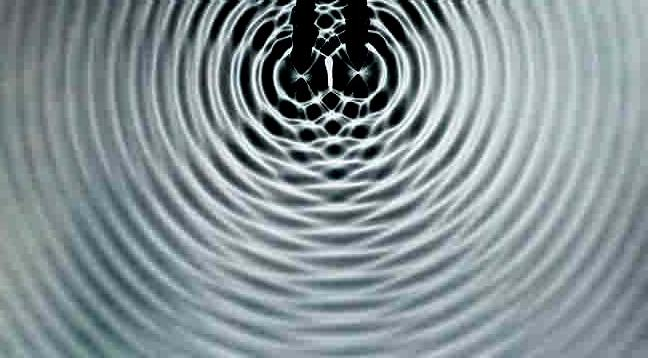
\includegraphics[scale=.6]{figure/9-23.jpg}
    \caption{水波的干涉图样}
\end{figure}

\textbf{频率相同的两列波叠加,使某些区域的振动加强,集些区域的振动减弱,并且振动加强和振动减弱的区域互相间隔,这种现象叫波的干涉},形成的图样叫\textbf{干涉图样}.

\textbf{不仅水波,一切波都能发生干涉,干涉是波特有的现象.}

如果两个波源的频率不同,或者两个波源没有固定的相差,那么它们发出的两列波互相叠加时,就不会出现稳定的加强区和减弱区,因为各点合振动的振幅是随时变化的,没有振动总是得到加强或总是得到减弱的区域,而都是有时振动加强,有时振动减弱,紊乱地振动着.这样的波源不能产生稳定的干涉现象,也就是不能形成干涉图样,所以,\textbf{要得到稳定的干涉现象,观察到干涉图样,两个波源必须是频率相同、相差恒定},这样的波源叫\textbf{相干波源}.对于水波等机械波,相干波源是容易得到的,但在研究其他波(例如光波)的干涉时,就不容易得到扣干波源,而必须采用巧妙的办法,到光学部分我们将会学到.

\subsection{波的衍射}

微风激起的水波,遇到突出水面的小石、芦苇,会绕过它们,继续传播,好象它们并不存在.在水波演示槽的水里放一个小障碍物,可以清楚地看到水波能绕过障碍物而继续传播.

\textbf{波绕过障碍物的现象,叫做波的衍射.}

是不是任何条件下都能发生波的衍射呢?
\begin{figure}[H]\centering
    \begin{tikzpicture}[>=stealth]
        \clip (-1.5, 0) rectangle (1.5,3);
        \foreach \x in {.1,.2,...,2}
            {
                \draw (-\x,0) arc (180:0:\x);
            }
        \draw[ultra thick] (-1.5,1)--(-.05,1);
        \draw[ultra thick] (1.5,1)--(.05,1);
        \fill [white](-1.5,1) rectangle (1.5, 2.2);
        \foreach \x in {.1,.2,...,3}
            {
                \draw (-\x,1) arc (180:0:\x);
            }
        \draw  [fill=black] (0,1)  circle (1pt);
        \draw[ultra thick] (-1.5, 0) rectangle (1.5,3);
        \draw  [fill=black] (0,0)  circle (1pt);
    \end{tikzpicture} \qquad
    \begin{tikzpicture}[>=stealth]
        \clip (-1.5, 0) rectangle (1.5,3);
        \foreach \x in {.1,.2,...,5}
            {
                \draw (-\x,0) arc (180:0:\x);
            }
        % \fill [white](-5.1,-2) rectangle (-1.5, 6);
        % \fill [white](1.5,-2) rectangle (5.1, 6);
        \draw[ultra thick] (-1.5,1)--(-.5,1);
        \draw[ultra thick] (1.5,1)--(.5,1);
        \draw [dotted](0,0)--(-.5,1)--(-1,2)--(-1.5,3);
        \draw [dotted](0,0)--(.5,1)--(1,2)--(1.5,3);
        % \fill [white](-1.5,3) rectangle (1.5, 6);
        \fill [white](-1.5,1)--(-.5,1)--(-1.5,3)--(-1.5,1);
        \fill [white](1.5,1)--(.5,1)--(1.5,3)--(1.5,1);
        \draw [ultra thick](-1.5, 0) rectangle (1.5,3);
        \draw  [fill=black] (0,0)  circle (1pt);
    \end{tikzpicture}
    \caption{波长相同的水波通过宽度不同的孔}
\end{figure}

我们利用水波演示槽观察水波通过孔的情形.在图9.24所示的两次实验中,水波的波长相同,孔的宽度不同.在孔的宽度跟波长差不多的情况下(图甲),孔后的整个区域里传播着以孔为中心的环形波,即发生了明显的衍射现象.在孔的宽度比波长大好多倍的情况下(图乙),在孔的后面,水波是在连接波源和孔边的两条直线所限制的区域里传播的,只在离孔比较远的地方,波才稍微弯绕到“影子”区域里.


可见,\textbf{能够发生明显的衍射现象的条件是:障碍物或孔的尺寸跟波长相差不多}.

\textbf{一切波都发生衍射,衍射也是波的特有现象}.
\newpage
\section{声学的初步知识}
\subsection{声波}
\subsubsection{声源}

声音在人类生活中具有重要意义,人类就是靠声
音传递语言、交流思想的.

声音是怎样发生的呢?\textbf{简单的观察告诉我们:一切发声
    的物体都在振动,它们就是声源.}
\begin{figure}[H]\centering
    \begin{tikzpicture}[>=stealth, scale=1.0]
        % \useasboundingbox(-0.5,1.34)rectangle(7.55,-1.47);
        \begin{scope}[yshift=-4cm,xshift=-0.8cm]
            \fill[gray](0.1,-0.45)rectangle(-0.1,-1.5);
            \fill[top color=lightgray,bottom color=gray](-0.4,0)arc(180:360:0.4)--++(0,0.3)--++(0.2,0)--++(0,-0.3)arc(0:-180:0.6)--++(0,0.3)--++(0.2,0)--cycle;
            \fill[bottom color=lightgray,top color=white](0.6,0.3)arc(0:10:13)--++(190:0.2)arc(10:0:12.8);
            \fill[bottom color=lightgray,top color=white](-0.4,0.3)arc(180:170:12.8)--++(170:0.2)arc(170:180:13);
            \fill[bottom color=lightgray,top color=gray](-0.4,0.3)arc(0:10:13)--++(190:0.2)arc(10:0:12.8);
            \fill[bottom color=lightgray,top color=gray](0.6,0.3)arc(180:170:12.8)--++(170:0.2)arc(170:180:13);
        \end{scope}
        \fill[bottom color=darkgray,top color=white](-0.5,0)rectangle(0.5,0.25);
        \draw[densely dashed](0,0)--(0,-2.0);
        \draw[thin](0,-0.5)arc(-90:-60:0.5)node[midway,below]{$\theta$};
        \draw[brown6](0,0)--(-60:1.7);
        \draw[->,red3](-60:1.7)--++(210:0.5);
        \fill[ball color=gray](-60:1.7)circle(5pt);
    \end{tikzpicture}
    \caption{发声的音叉在振动}
\end{figure}

用橡皮槌敲音叉,使它发声.如
果把悬在线上的小球跟发声的音叉接
触,小球会被弹开(图9.25).用手指
轻轻接触发声的音叉,可以直接感觉
到它的振动,如果捏紧音叉的叉股,
使它停止振动,我们就听不到声音了.

锣、鼓是靠锣面、鼓膜的振动发声
的,锣、鼓发声的时候,如果用手轻触
锣面或鼓膜,可以直接感觉到它们的振动.弦乐器是靠弦的
振动发声的.观察发声的弦,会看到它的轮廓变得模糊了,
这是因为弦在很快振动的缘故.人是靠声带的振动发声的.
我们说话的时候,如果用手摸咽喉,就会感觉到振动.

不但音叉、锣面、鼓膜、弦等固体能够振动发声,气体和液
体也能够振动发声,各种管乐器就是靠空气柱的振动发声的.

\subsubsection{声波}

声源振动的时候,在空气中形成声波.声源,例如
振动的音叉,它的叉股向一侧振动时,压缩邻近的空气,使这
部分空气变密,叉股向相反方向振动对,这部分空气又变疏.
这种疏密相间的状态由声源向外传播(图9.26),形成声波.
传入人耳,使鼓膜振动,就引起声音的感觉.
\begin{figure}[H]\centering
    \begin{tikzpicture}[>=stealth, scale=1.0]
        % \useasboundingbox(-0.5,1.34)rectangle(7.55,-1.47);
        \foreach \x in {0.3,2.8,5.3}
            {
                \fill[left color=cyan!90!lightgray,right color=cyan!90!lightgray,middle color=cyan!40!lightgray!50](\x,0)rectangle++(2.5,1.2);
            }
        % \draw(0.3,0)rectangle(8,1.2);
        \begin{scope}[scale=0.55]
            \fill[gray](0.1,-0.45)rectangle(-0.1,-1.5);
            \fill[top color=lightgray,bottom color=gray](-0.4,0)arc(180:360:0.4)--++(0,0.3)--++(0.2,0)--++(0,-0.3)arc(0:-180:0.6)--++(0,0.3)--++(0.2,0)--cycle;
            \fill[bottom color=lightgray,top color=white](0.6,0.3)arc(0:10:13)--++(190:0.2)arc(10:0:12.8);
            \fill[bottom color=lightgray,top color=white](-0.4,0.3)arc(180:170:12.8)--++(170:0.2)arc(170:180:13);
            \fill[bottom color=lightgray,top color=gray](-0.4,0.3)arc(0:10:13)--++(190:0.2)arc(10:0:12.8);
            \fill[bottom color=lightgray,top color=gray](0.6,0.3)arc(180:170:12.8)--++(170:0.2)arc(170:180:13);
        \end{scope}
        \draw[fill=pink!20!orange!10](8.549,0.815)..controls(8.525,1.170)and(8.153,1.330)..
        (7.974,0.940)..controls(7.879,0.752)and(7.976,0.454)..
        (8.166,0.247)..controls(8.406,0.004)and(8.438,0.034)..
        (8.520,0.078)..controls(8.616,0.139)and(8.511,0.240)..(8.587,0.296);
        \draw
        (8.242,0.296)..controls(7.999,0.615)and(8.034,0.831)..
        (8.125,0.956)..controls(8.169,1.039)and(8.289,1.062)..
        (8.354,1.028)..controls(8.424,0.997)and(8.440,0.976)..
        (8.402,0.899)..controls(8.374,0.827)and(8.477,0.644)..(8.209,0.641)
        (8.385,0.829)..controls(8.346,0.716)and(8.204,0.731)..
        (8.197,0.613)..controls(8.195,0.575)and(8.200,0.543)..
        (8.217,0.506)..controls(8.241,0.383)and(8.344,0.472)..
        (8.428,0.385)..controls(8.509,0.287)and(8.567,0.349)..
        (8.496,0.429)..controls(8.426,0.485)and(8.467,0.557)..(8.415,0.599)
        (8.217,0.506)..controls(8.234,0.583)and(8.460,0.558)..(8.488,0.700)
        (8.398,0.939)..controls(8.315,0.953)and(8.270,0.858)..(8.302,0.800);

    \end{tikzpicture}
    \caption{空气中的声波}
\end{figure}

因为空气质点的振动方向与声波的传播方向在同一直线上,所以\textbf{声波是纵波}.

声波不仅能在气体中传播,在固体和液体中也能够传播.在桌而的一端放一只表,把耳朵贴在桌面的另一端,可以听到从桌面传来的表的走动声,让螺丝刀跟机器的外壳接触,把耳朵贴在螺丝刀的把上,可以听到机器内部的声音.人潜没在水里,可以听到岸上的声音,鱼能够听到岸上人的脚步声和说话声,这个事实喜欢钓鱼的人知道得很清楚.

\begin{table}[H]
    \centering
    \caption{0$^\circ { C}$时几种媒质中的声波传播速率(${ m/s}$)}
    \begin{tabularx}{\textwidth}{MMMM}
        \toprule[1.5pt]
        媒质 & 声速   & 媒质 & 声速        \\
        \midrule
        空气 & 332  & 玻璃 & 5000—6000 \\
        水  & 1450 & 松木 & 3320      \\
        铜  & 3860 & 软木 & 430—530   \\
        铁  & 4900 & 橡胶 & 30—50     \\
        \bottomrule[1.5pt]
    \end{tabularx}
\end{table}

声波在不同媒质中的传播速率是不同的,声波在0$^\circ { C}$空气里的传播速率是332$\si{m/s}$,20$^\circ { C}$时是344$\si{m/s}$,30$^\circ { C}$时是349$\si{m/s}$.声波在水里的传播速率大约是空气里的四倍半,在金属里传播速率更大.

\subsection{某些声音现象}
\subsubsection{声波的反射}

声波遇到障碍物会被反射回来,反射回来的声波传入人耳,我们就听到回声.对着山崖或高大的建筑物喊一声,就可以所到清晰的回声,北京天坛公园的回音壁(图9.27)就利用了声波反射的道理,回音壁是明代修建的,已有三百多年的历史,它是一个圆形的墙壁,直径有65米(图9.28),一个人对着回音壁说话,他发出的声波沿着回音壁多次反射,另一个人贴近回音壁可以听到前一个人说的话,回音壁的修建充分显示了我国劳动人民的智慧.
\begin{figure}[H]
    \begin{floatrow}
        \ffigbox[0.45\textwidth]{
            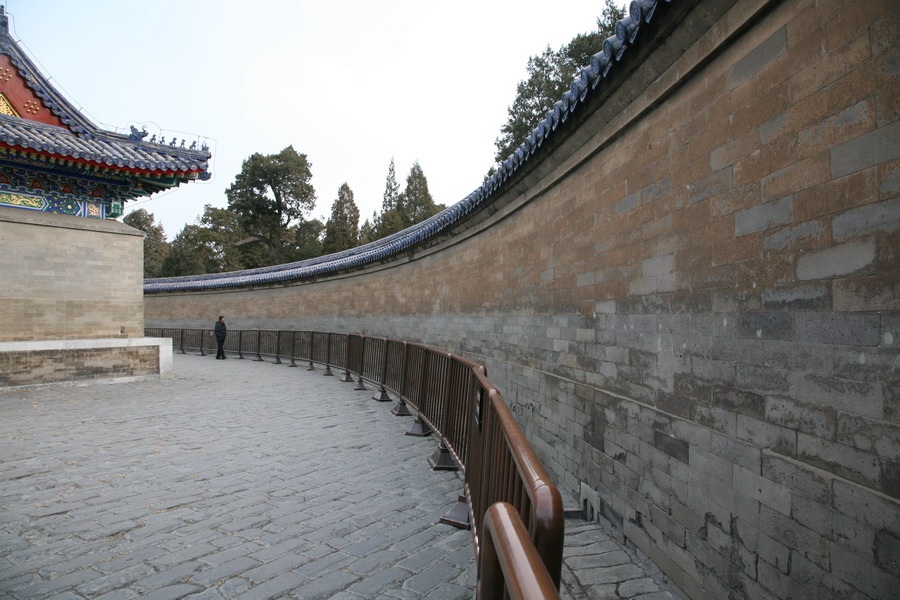
\includegraphics[scale=0.25]{figure/9-27.jpg}
        }{\caption{回音壁}}
        \ffigbox[0.5\textwidth]{
            \begin{tikzpicture}[>=latex,scale=1.0]
                \useasboundingbox(-2.8,2.8)rectangle(2.8,-2.9);
                \draw[fill=gray](250:2.8)arc(250:-70:2.8)--++(110:0.1)arc(-70:250:2.7)--cycle;
                \foreach \x in {-0.9,-0.85,...,0.9}
                    {
                        \draw[very thin](\x,1.7)--++(0,-0.2);
                    }
                \draw(-0.95,1.45)rectangle(0.95,1.75)(-0.95,1.5)rectangle(0.95,1.7);
                \foreach \x in {0.7,0.75,...,1.0}
                    {
                        \draw[very thin](-0.1,\x)--(0.1,\x);
                    }
                \draw(-0.15,0.65)rectangle(0.15,1.0)(-0.1,0.65)rectangle(0.1,1.0);
                \draw[outer color=yellow!40!orange,inner color=white](0,1.6)circle(0.7);
                \foreach \x in {0,10,...,350}{ \draw([shift=(\x:0.05)]0,1.6)--++(\x:0.6);}
                \foreach \x in {1.05,1.1,...,1.3}
                    {
                        \draw[very thin](\x,-0.3)--(\x,-0.5);
                        \draw[very thin](-\x,-0.3)--(-\x,-0.5);
                    }
                \draw(-1.3,-0.3)rectangle(-1,-0.5)(1.3,-0.3)rectangle(1,-0.5);
                \draw(-1.3,-0.25)rectangle(-1,-0.55)(1.3,-0.25)rectangle(1,-0.55);
                \foreach \x in {-1.5,1.5}
                    {
                        \draw[top color=yellow!40!orange,bottom color=yellow!40!orange,middle color=yellow!40](\x-0.25,0.4)rectangle(\x+0.25,-1.2);
                        \foreach \y in {-0.2,-0.15,...,0.2}{\draw[very thin](\x+\y,0.4)--(\x+\y,-1.2);}
                        \draw[left color=yellow!40!orange,right color=yellow!40!orange,middle color=yellow!40](\x-0.25,0.4)--(\x-0.25,-1.2)--(\x,-1.0)--(\x+0.25,-1.2)--(\x+0.25,0.4)--(\x,0.2)--cycle;
                        \draw(\x,0.2)--(\x,-1.0);
                        \foreach \y in {-8,-7,...,8}
                            {
                                \draw[very thin] (\x,-0.4+\y*0.075)--(\x+0.25,-0.4+\y*0.1);
                                \draw[very thin] (\x,-0.4+\y*0.075)--(\x-0.25,-0.4+\y*0.1);
                            }
                    }
                \draw[postaction={decorate},decoration={markings,mark=between positions 0.125 and 0.9 step 0.25 with {\arrow{>}} }](-20:2.7)\foreach \x in {40,100,...,260}{--(\x:2.7)};
                \draw[postaction={decorate},decoration={markings,mark=between positions 0.0833 and 0.92 step 0.167 with {\arrow{>}} }](-20:2.7)\foreach \x in {20,60,...,220}{--(\x:2.7)};
                \draw[postaction={decorate},decoration={markings,mark=at position 0.5 with {\arrow{>}} }](-65:2.7)--(-20:2.7);
                \draw[->](-20:2.7)--(1.75,-1.1);
                \draw[->](-20:2.7)--(1.75,-0.3);
                \draw[->](-20:2.7)--(1.75,0.3);
                \draw[fill=gray](-0.9,-2.65)rectangle(0.9,-2.55);
                \foreach \x in {-0.7,0,0.7}
                    {
                        \foreach \y in {-2.8,-2.75,...,-2.6}
                            {
                                \draw[very thin](\x-0.075,\y)--(\x+0.075,\y);
                            }
                        \draw(\x-0.075,-2.85)rectangle(\x+0.075,-2.6);
                        \draw(\x-0.1,-2.85)rectangle(\x+0.1,-2.6);
                        \draw[left color=yellow!40!orange,right color=yellow!40!orange,middle color=white](\x-0.25,-2.7)rectangle(\x+0.25,-2.5);
                        \draw[top color=yellow!40!orange,bottom color=yellow!40!orange,middle color=yellow!40](\x-0.25,-2.7)--(\x+0.25,-2.7)--(\x+0.15,-2.6)--(\x+0.25,-2.5)--(\x-0.25,-2.5)--(\x-0.15,-2.6)--cycle;
                        \draw(\x-0.15,-2.6)--(\x+0.15,-2.6);
                    }
            \end{tikzpicture}
        }{\caption{声波沿着回音壁多次反射}}
    \end{floatrow}
\end{figure}

反射回来的声波要在原来的声波消失后至少经过0.1秒到达人耳,我们才能把回声和原来的声音区分开.如果反射声波的障碍物离我们很近,回声就跟原来的声音混在一起,使原来的声音加强,在门窗关闭的屋子里谈话,听起来比在旷野里响,就是这个道理.

声波在室内传播时,要被墙壁、天花板、地板等障碍物反射,每反射一次还要被障碍物吸收一些,这样,当声源停止发声后,声波在室内要经过多次反射和吸收,最后才消失,我们就感觉到声源停止发声后声音还继续一段时间.这段时间叫做交混回响时间,交混回响时间的长短是音乐厅、病院、礼堂等建筑物的重要声学特性,交混回响时间过长,前音未落后音又起,互相重叠,分辨不清;交混回响时间过短,给人以单调、不丰满的感觉,不适于演奏.北京首都剧场的交混回响时间,满座时是1.36秒,空座时是3.3秒,北京人民大会堂的交混回响时间,满座时是1.6秒,空座时是3秒.

\subsubsection{声波的干涉}

声波也能发生干涉,这可以用音叉来演示.
音叉发声的时候,它的两个叉股是两个相同的波源,它们产生
的两列波发生干涉,出现相间的加强区和减弱区.在加强区,
空气的振动加强,我们听到的声音也强;在减弱区,空气的振
动减弱,我们听到的声音也弱.因此,当我们环绕正在发声的
音叉走一周,或者人不动而使音叉绕叉柄的纵轴旋转,就会听
到声音忽强忽弱.

\subsubsection{声波的衍射}

闻其声而不见其人,这是司空见惯的现象.
怎样解释这种现象呢?一切波都能发生衍射,只是由于波长不
同,在通常条件下,有的会发生明显的衍射,有的表现为直线
传播.我们能听到的声波,波长在17厘米到17米的范围内,
是可以跟一般障碍物的尺寸相比的,所以能绕过一般障碍物,
使我们听到障碍物另一侧的声音.而光的波长,到光学部分
将会学到,约在0.4到0.8微米的范围内,跟一般障碍物的尺
寸相比非常非常小,所以几乎不发生衍射,这就是闻其声而不
见其人的原因.


\subsubsection{声音的共鸣}


声音的共振现象叫\textbf{共鸣}.取两只频率相同
的音叉并列放在一起,敲响共中的一只,然后用手按住使它停
止振动,就可以听到没有被敲的那只音叉发出了声音.被敲
响的那只音叉振动时发出声波,传到另一只音叉,对它产生周
期性作用力,使它做受迫振动.由于两只音叉的频率相等,后
一只音叉受到的周期性作用力的频率跟它的固有频率相等,
所以后一只音叉产生了最大振幅的受迫振动,也就是发生了
共鸣,如果两只音叉的频率不同,受迫振动比较弱,不会发生
共鸣,这时按住敲响的音叉使它停止振动,就听不到另一只音
叉的声音了.
\begin{figure}[H]\centering
    \begin{tikzpicture}[>=stealth,scale=0.82]
        \begin{scope}[rotate=-90,yshift=-0.7cm,xshift=-5.8cm,scale=0.4,
            ]
            \fill[gray](0.1,-0.45)rectangle(-0.1,-1.5);
            \fill[top color=lightgray,bottom color=gray](-0.4,0)arc(180:360:0.4)--++(0,0.3)--++(0.2,0)--++(0,-0.3)arc(0:-180:0.6)--++(0,0.3)--++(0.2,0)--cycle;
            \fill[bottom color=lightgray,top color=white](0.6,0.3)arc(0:10:13)--++(190:0.2)arc(10:0:12.8);
            \fill[bottom color=lightgray,top color=white](-0.4,0.3)arc(180:170:12.8)--++(170:0.2)arc(170:180:13);
            \fill[bottom color=lightgray,top color=gray](-0.4,0.3)arc(0:10:13)--++(190:0.2)arc(10:0:12.8);
            \fill[bottom color=lightgray,top color=gray](0.6,0.3)arc(180:170:12.8)--++(170:0.2)arc(170:180:13);
            \draw[lightgray](1.0,1.0)to[bend right](1.0,2.5);
            \draw[lightgray](1.2,0.9)to[bend right](1.2,2.6);
            \draw[lightgray](1.4,0.8)to[bend right](1.4,2.7);
            \draw[lightgray](-1.0,1.0)to[bend left](-1.0,2.5);
            \draw[lightgray](-1.2,0.9)to[bend left](-1.2,2.6);
            \draw[lightgray](-1.4,0.8)to[bend left](-1.4,2.7);
        \end{scope}
        \draw[lightgray](-0.1,1.7)--(-0.1,3)(0.1,1.7)--(0.1,3)(0,1.7)ellipse(0.1 and 0.05);
        \fill[cyan!20,opacity=0.5](0,3)ellipse(2.0 and 0.8);
        \fill[cyan!50,opacity=0.5](2.0,1.0)--++(0,2)arc(360:180:2.0 and 0.8)--++(0,-2)arc(180:360:2.0 and 0.8);
        \draw[very thick,lightgray!80](0,1)ellipse(2.0 and 0.8)(0,3.5)ellipse(2.0 and 0.8)(-2,1)--(-2,3.5)(2,1)--(2,3.5);
        \fill[white,opacity=0.7](-0.1,3)--(-0.1,5)arc(180:0:0.1 and 0.05)--(0.1,3)arc(360:180:0.1 and 0.05);
        \draw[darkgray](-0.1,3)--(-0.1,5)(0.1,3)--(0.1,5)(0,3)ellipse(0.1 and 0.05)(0,5)ellipse(0.1 and 0.05);
        \draw[|<->|](0.6,3)--(0.6,5)node[midway,right]{$L$};
    \end{tikzpicture}
    \caption{空气柱的共鸣}
\end{figure}

音叉和空气柱也可以发生共鸣.在盛水的容器中插一根
粗玻璃管,在管口的上方放一个
正在发声的音叉(图9.29),慢
慢把玻璃管提上来,以增大玻璃
管中空气柱的长度.当空气柱的
长度增大到一定值时,空气柱的
固有频率与音叉的频率相等,空
气柱跟音叉发生共鸣,我们可以
听到相当强的声音.可以证明:
跟某一声波共鸣的空气柱的最短长度等于该声波波长的1/4.
因此,利用空气柱的共鸣可以测定声波的波长.


\subsection*{练习九}

\begin{enumerate}
    \item 第一次测定声音在水中的传播速率是1827年在日
          内瓦湖上用下面的方法进行的:在一只船上实验员向水里放
          下一个钟,当敲这个钟的时候,使船上的火药同时发光;在另
          一只船上,另一实验员向水里放下一个听音器,他测量从看到
          火药闪光到听到钟声所经过的时间.

          两船相距14千米,看到火药闪光后10秒钟听到声音,求
          声音在水中的传播速率.

    \item 第一次测定铸铁里的声速是在巴黎用下面的方法进
          行的:从铸铁管的一端敲一下钟,在管的另一端听到两次响
          声,第一次是由铸铁管传来的,第二次是由空气传来的.管长
          931米,两次响声相隔2.5秒,如果当时空气中的声速是340
          $\si{m/s}$,求铸铁中的声速.

    \item 为了听到回声,反射声波的障碍物至少应该离开我
          们多远?猎人在射击后6秒钟听到射击的回声,障碍物离猎人
          有多远?设空气中的声速是340$\si{m/s}$.
    \item 人能听到的声膏的最高频率是20000赫.狗能听到
          的声音的最高频率是50000赫.蝙蝠能发出并且能听到的声
          音频率高达120000赫.分别求出人、狗、蝙蝠能听到的,在
          0$^{\circ}$C空气中传播的声波的最短波长.
    \item 在一次如图9.29所示的空气柱共鸣的实验中,测得
          共鸣时空气柱的最短长度为19厘米,声波的波长有多长?已
          知音叉的频率是440赫,空气中的声速有多大?


\end{enumerate}

\subsection{音调、响度、音品}
\subsubsection{乐音和噪声}

根据人的感觉,通常把声音分为两类:乐音和噪声.

好听悦耳的声音叫做乐音,乐音是由做周期性振动的声
源(如音叉、乐器、歌唱家的喉咙等)发出来,它的波形曲线
是周期性的曲线(图9.30).
\begin{figure}[H]\centering
    \begin{tikzpicture}[>=stealth]
        \useasboundingbox(-0.05,1.34)rectangle(8.05,-1.47);
        \foreach \x in {0,1.6,...,8}
            {
                \begin{scope}[xshift=\x cm]
                    \draw[thick]
                    (0.000, 0.000)..controls(0.008, 1.572)and(0.048, 1.637)..
                    (0.055, 0.745)..controls(0.058, 0.232)and(0.120, 0.319)..
                    (0.135, 0.442)..controls(0.148, 0.550)and(0.188, 0.527)..
                    (0.196, 0.456)..controls(0.204, 0.409)and(0.242, 0.293)..
                    (0.273, 0.568)..controls(0.295, 0.768)and(0.364, 0.867)..
                    (0.391, 0.418)..controls(0.428, 0.057)and(0.483, 0.061)..
                    (0.521, 0.167)..controls(0.539, 0.219)and(0.569, 0.329)..
                    (0.618, 0.020)..controls(0.662,-0.283)and(0.721,-0.489)..
                    (0.763,-0.067)..controls(0.824, 0.390)and(0.853, 0.047)..
                    (0.874,-0.098)..controls(0.921,-0.420)and(0.970,-0.439)..
                    (1.016,-0.288)..controls(1.079,-0.111)and(1.131,-0.315)..
                    (1.136,-0.534)..controls(1.169,-1.170)and(1.227,-0.949)..
                    (1.231,-0.815)..controls(1.239,-0.671)and(1.263,-0.618)..
                    (1.274,-0.704)..controls(1.280,-0.751)and(1.364,-0.832)..
                    (1.405,-0.547)..controls(1.445,-0.268)and(1.477,-0.322)..
                    (1.506,-0.900)..controls(1.530,-1.838)and(1.588,-1.621)..(1.600, 0.000);
                \end{scope}
            }
    \end{tikzpicture}
    \caption{乐音的波形曲线}
\end{figure}

嘈杂刺耳的声音叫做噪声.劈木材时的破裂声、街道上
的嘈杂声、工厂里机器的轧轧声,都是噪声.噪声是由做无规
则的非周期性振动产生的,波形曲线非常复杂,是无规则的
非周期性曲线(图9.31).
\begin{figure}[H]\centering
    \begin{tikzpicture}[>=stealth]
        \draw(0,0)--(12,0);
        \draw[thick,line join=round]( 0.397,-0.036)--( 0.460, 0.031)--( 0.484, 0.499)--( 0.592,-0.237)--( 0.702, 0.376)--( 0.783, 0.437)--( 0.837, 0.326)--( 0.899,-0.077)--( 0.986,-0.164)--( 1.053,-0.086)--( 1.042, 0.037)--( 1.167, 0.053)--( 1.196, 0.343)--( 1.229, 0.370)--( 1.301, 0.142)--( 1.367, 0.160)--( 1.479, 0.422)--( 1.546, 0.477)--( 1.602, 0.455)--( 1.632, 0.321)--( 1.675,-0.101)--( 1.688,-0.219)--( 1.740,-0.259)--( 1.835,-0.195)--( 1.875, 0.072)--( 1.889, 0.219)--( 1.911, 0.319)--( 1.976, 0.211)--( 2.041, 0.289)--( 2.044, 0.384)--( 2.135, 0.038)--( 2.229, 0.249)--( 2.274, 0.036)--( 2.303,-0.086)--( 2.375,-0.132)--( 2.404,-0.227)--( 2.415,-0.350)--( 2.435,-0.430)--( 2.508,-0.362)--( 2.533,-0.195)--( 2.541,-0.034)--( 2.533, 0.132)--( 2.514, 0.395)--( 2.543, 0.520)--( 2.614, 0.459)--( 2.612, 0.308)--( 2.629, 0.111)--( 2.641, 0.046)--( 2.714, 0.334)--( 2.813,-0.070)--( 2.897, 0.325)--( 3.086,-0.503)--( 3.341, 0.397)--( 3.486,-0.079)--( 3.637, 0.292)--( 3.723, 0.216)--( 3.847, 0.315)--( 3.999,-0.062)--( 4.072, 0.184)--( 4.145, 0.054)--( 4.267, 0.265)--( 4.373,-0.290)--( 4.507, 0.265)--( 4.603, 0.154)--( 4.692,-0.241)--( 4.758, 0.176)--( 4.820, 0.250)--( 4.955, 0.143)--( 5.030, 0.144)--( 5.119,-0.133)--( 5.169,-0.242)--( 5.229,-0.054)--( 5.229, 0.118)--( 5.232, 0.326)--( 5.309, 0.259)--( 5.392, 0.307)--( 5.445, 0.170)--( 5.559, 0.173)--( 5.642,-0.144)--( 5.709,-0.257)--( 5.788,-0.167)--( 5.817, 0.198)--( 5.928, 0.200)--( 5.953, 0.289)--( 6.071, 0.422)--( 6.131, 0.342)--( 6.172, 0.099)--( 6.229,-0.056)--( 6.282,-0.302)--( 6.359,-0.295)--( 6.390, 0.265)--( 6.513, 0.191)--( 6.608, 0.216)--( 6.628, 0.389)--( 6.685, 0.427)--( 6.724, 0.308)--( 6.739,-0.068)--( 6.804,-0.248)--( 6.927,-0.149)--( 7.035,-0.313)--( 7.102,-0.266)--( 7.095, 0.069)--( 7.172, 0.219)--( 7.190, 0.400)--( 7.242, 0.412)--( 7.267, 0.119)--( 7.355, 0.039)--( 7.414,-0.359)--( 7.522,-0.099)--( 7.646, 0.177)--( 7.757,-0.094)--( 7.847, 0.119)--( 7.909,-0.083)--( 8.014, 0.127)--( 8.156,-0.119)--( 8.253, 0.328)--( 8.280, 0.340)--( 8.341, 0.261)--( 8.429, 0.391)--( 8.473, 0.370)--( 8.458,-0.302)--( 8.552, 0.039)--( 8.630,-0.315)--( 8.671,-0.287)--( 8.713, 0.321)--( 8.789,-0.283)--( 8.875, 0.171)--( 8.927,-0.283)--( 9.037, 0.194)--( 9.094, 0.181)--( 9.163,-0.072)--( 9.210,-0.307)--( 9.290,-0.270)--( 9.331,-0.138)--( 9.338,-0.039)--( 9.361, 0.181)--( 9.530, 0.376)--( 9.540, 0.205)--( 9.509, 0.017)--( 9.525,-0.225)--( 9.686,-0.040)--( 9.755, 0.239)--( 9.817, 0.298)--( 9.865, 0.120)--( 9.892,-0.077)--( 9.915,-0.214)--( 9.980,-0.222)--(10.041,-0.025)--(10.090, 0.129)--(10.164, 0.044)--(10.212,-0.281)--(10.284,-0.250)--(10.384, 0.271)--(10.420, 0.305)--(10.471, 0.213)--(10.523, 0.228)--(10.572, 0.289)--(10.594, 0.054)--(10.620,-0.060)--(10.712,-0.029)--(10.768,-0.096)--(10.835,-0.042)--(10.833, 0.152)--(10.996, 0.345)--(11.042,-0.265)--(11.093,-0.271)--(11.132,-0.059)--(11.192, 0.080)--(11.236,-0.058)--(11.272,-0.142)--(11.363,-0.067)--(11.410, 0.090)--(11.477, 0.109)--(11.526, 0.016)--(11.551,-0.059)--(11.701, 0.029);
    \end{tikzpicture}
    \caption{噪声的波形曲线}
\end{figure}


乐音具有音调、响度、音品三种特性,下面分别加以介绍.

\subsubsection{音调}


所谓音调是指声音的高低、按照一个歌谱来唱
歌,“7”的音调就比“3”的音调高.一般说来,儿童的音调比成
人高,女人的音调比男人高.

取两只完全相同的音叉,在一只的叉股上裹一小条铜片.
用同样大小的力敲这两只音叉,听起来没包铜片的音调高,包
了铜片的音调低.仔细观察它们的振动会发现,音调高的振
动得快,频率大;音调的振动得慢,频率小.如果眼晴区分
不清音叉振动的快慢,还可以做图9.32所示的实验.装在同
一根轴上的四个齿轮,自上而下,齿数分别为80、60、50、40.
当这四个齿轮一起旋转时,用一张硬纸片依次接触这四个齿
轮,会听到纸片依次发出四个音调,齿轮的齿数越多,接触它
的纸片振动得越快,即频率越大,音调就越高.
\begin{figure}[H]
    \centering
    \begin{tikzpicture}[>=stealth]
        \newcommand{\hand}[2][0]{
            \begin{scope}[#2,rotate=#1,on background layer]
                \fill[pink!10!orange!10,draw=black,very thin]
                (-0.812, 0.563)..controls(-0.430, 0.531)and(-0.584, 0.282)..(-0.179, 0.197)..controls( 0.040, 0.131)and( 0.113, 0.007)..( 0.141,-0.072)--( 0.916,-0.020)..controls( 0.915, 0.319)and( 0.727, 0.379)..( 0.640, 0.609)..controls( 0.541, 0.843)and( 0.383, 0.790)..( 0.209, 0.818)..controls(-0.074, 0.877)and(-0.176, 0.901)..(-0.408, 1.006);
                \draw[very thin]
                (0.122, 0.128)..controls(0.235, 0.126)and(0.288, 0.186)..(0.542, 0.499)
                (0.459, 0.245)..controls(0.460, 0.199)and(0.559, 0.216)..(0.625, 0.410);
            \end{scope}
            \begin{scope}[#2,rotate=#1]
                \fill[pink!10!orange!10,draw=black,very thin]
                (-0.181, 0.373)..controls(-0.099, 0.290)and(-0.074, 0.245)..(-0.020, 0.228)..controls( 0.056, 0.195)and( 0.200, 0.208)..( 0.287, 0.139)..controls( 0.388, 0.065)and( 0.452,-0.156)..( 0.534,-0.196)..controls( 0.648,-0.315)and( 0.893,-0.305)..( 0.826,-0.169)..controls( 0.765,-0.009)and( 0.684, 0.104)..( 0.649, 0.152)..controls( 0.542, 0.285)and( 0.496, 0.354)..( 0.392, 0.463);
                \draw[very thin](0.772,-0.261)..controls(0.750,-0.255)and(0.726,-0.218)..
                (0.709,-0.192)..controls(0.677,-0.141)and(0.705,-0.102)..(0.758,-0.065)
                (0.595,-0.024)..controls(0.606,-0.008)and(0.640, 0.002)..(0.641, 0.022)
                (0.551, 0.047)..controls(0.596, 0.055)and(0.628, 0.092)..(0.632, 0.120);
            \end{scope}
        }
        %%% 纸
        \draw[fill=yellow9!10!white](-2.3,2.3)to[bend left=5](-0.8,2.3)--(-0.8,1.4)to[bend right=5](-2.3,1.4)--cycle;
        %%% 机床
        \fill[left color=darkgray,right color=darkgray,middle color=white](0.4,-1.7)rectangle(0.6,-1.0);
        \fill[left color=darkgray,right color=darkgray,middle color=white]
        (-0.5,-1.1)arc(180:261:0.5 and 0.3)--(1,-1.5)--(1,-1.4)--(-0.0791,-1.2962)arc(261:180:0.5 and 0.3)--(-0.5,-1)--cycle;
        \fill[lightgray](1,-0.6)--(-0.0791,-0.7038)arc(99:261:0.5 and 0.3)--(1,-1.4);
        \draw[ultra thick,brown!80!black](-0.1,-0.9)--(1,-0.7);
        \fill[left color=darkgray,right color=darkgray,middle color=white](0,-1.0)ellipse(0.1 and 0.06);
        \fill[left color=darkgray,right color=darkgray,middle color=white](0.1,-0.6)rectangle(-0.1,-1.0);
        \fill[left color=darkgray,right color=darkgray,middle color=white](0,-0.7)ellipse(0.2 and 0.12);
        \fill[left color=darkgray,right color=darkgray,middle color=white](0.2,-0.6)rectangle(-0.2,-0.7);
        \fill[left color=white,right color=darkgray,middle color=lightgray](0,-0.82)..controls(0.2,-0.82)and(0.2,-0.76)..(0.4,-0.76)--(0.5,-1.06)--(1.0,-1.06)--(1.0,-0.96)--(0.7,-0.96)--(0.6,-0.66)--(0.4,-0.64)..controls(0.2,-0.64)and(0.2,-0.58)..(0,-0.58);
        \fill[darkgray!80](0,-0.72)..controls(0.2,-0.72)and(0.2,-0.66)..(0.4,-0.66)--(0.4,-0.54)..controls(0.2,-0.54)and(0.2,-0.48)..(0,-0.48);
        \fill[darkgray!80](0.4,-0.66)rectangle(0.6,-0.54)(0.7,-0.96)rectangle(1.0,-0.84);
        \fill[darkgray!80!black](0.6,-0.66)--(0.6,-0.54)--(0.7,-0.84)--(.7,-0.96);
        \fill[darkgray!80](0,-0.6)ellipse(0.2 and 0.12);
        \fill[left color=darkgray,right color=darkgray,middle color=white](0,-0.6)ellipse(0.1 and 0.06);
        \fill[left color=darkgray,right color=darkgray,middle color=white](0.1,-0.5)rectangle(-0.1,-0.6);
        \fill[darkgray!80](0,-0.5)ellipse(0.1 and 0.06);
        \fill[left color=gray,right color=gray,middle color=white](0,-0.5)ellipse(0.05 and 0.03);
        \fill[left color=gray,right color=gray,middle color=white](-0.05,-0.5)rectangle(0.05,0);
        \draw[ultra thick,brown!80!black](-0.1,-0.9)--(1,-1.1);
        %%% 齿轮
        \draw[decorate,decoration={zigzag,segment length=1.4mm,amplitude=0.16mm},fill=lightgray!50](0,0) ellipse (1 and 0.32);
        \fill[darkgray!80](0,0)ellipse(0.1 and 0.06);
        \fill[left color=gray,right color=gray,middle color=white](0,0)ellipse(0.05 and 0.03);
        \fill[left color=gray,right color=gray,middle color=white](-0.05,0)rectangle++(0.1,0.5);
        \draw[decorate,decoration={zigzag,segment length=1.1mm,amplitude=0.14mm},fill=lightgray!50](0,0.5) ellipse (1 and 0.32);
        \fill[darkgray!80](0,0.5)ellipse(0.1 and 0.06);
        \fill[left color=gray,right color=gray,middle color=white](0,0.5)ellipse(0.05 and 0.03);
        \fill[left color=gray,right color=gray,middle color=white](-0.05,0.5)rectangle++(0.1,0.5);
        \draw[decorate,decoration={zigzag,segment length=0.8mm,amplitude=0.12mm},fill=lightgray!50](0,1) ellipse (1 and 0.32);
        \fill[darkgray!80](0,1.0)ellipse(0.1 and 0.06);
        \fill[left color=gray,right color=gray,middle color=white](0,1.0)ellipse(0.05 and 0.03);
        \fill[left color=gray,right color=gray,middle color=white](-0.05,1.0)rectangle++(0.1,0.5);
        \draw[decorate,decoration={zigzag,segment length=0.5mm,amplitude=0.1mm}, fill=lightgray!50](0,1.5) ellipse (1 and 0.32);
        \fill[darkgray!80](0,1.5)ellipse(0.1 and 0.06);
        \fill[left color=gray,right color=gray,middle color=white](0,1.5)ellipse(0.05 and 0.03);
        \fill[left color=gray,right color=gray,middle color=white](-0.05,1.5)rectangle++(0.1,0.1);
        \fill[gray!20](0,1.6)ellipse(0.05 and 0.03);
        \draw[thin,->](1.2,0)arc(0:-40:1.2 and 0.4);
        \draw[thin,->](-1.2,0)arc(180:140:1.2 and 0.4);
        \hand{xshift=-2.3cm,yshift=2.3cm}
    \end{tikzpicture}
    \caption{纸片振动得越快,发出的声音越高}
\end{figure}

上面的实验告诉我们:人们对音调的感觉客观上决定于
振动的频率.频率不同,产生的效果也不同,频率越大,音调
就越高,

我们的耳朵能够听到的声音的频率范围是从20赫到
20000赫,在自然界和技术中也存在着频率低于20赫和高
于20000赫的声波,但是它们不能引起声音的感觉,所以我们
听不到它们.


\subsubsection{响度}
所谓响度是指声音的强弱.用力敲锣或打鼓,发
出的声音强,即响度大;轻轻敲锣或打鼓,发出的声音弱,即
响度小.用橡皮锤重敲一下音叉,发出的声音的响度大;轻敲
一下,发出的声音的响度小,仔细观察锣鼓或音叉的振动情况
会发现,重敲的时候,声源振动的振幅大,发出的声音听起来
响度大.可见,振动的振幅不同,产生的效果也不同.

声源的振幅越大,声波传递的能量越多,或者确切地说,
单位时间内通过垂直于声波传播方向的单位面积的能量越
多.在声学中,单位时间内通过垂直于声波传播方向的单位
面积的能量叫做\textbf{声强}.人们对响度的感觉客观上决定于
声强.

对于频率在20—20000赫这个范围内的声波,声强过小
将听不到声音,声强过大又震耳难忍.要引起听觉,声强也有
一个范围,而且这个范围的大小对不同频率的声波来说并不
相同.对人耳最敏感的声波的频率在3000赫左右,在这个频
率附近引起听觉的声强范围最大,这个范围大约是从
$10^{-12}{ W}/{ m^2}$
到$1{ W}/{ m^2}$.

\subsubsection{音品}

胡琴、提琴、钢琴、黑管等不同乐器发出来的声音
各有特色,即使音调和响度都相同,我们也能把它们分辨开,
我们说它们的音品不同.

音品是由什么决定的呢?

实验表明:音叉的振动是简谐振动,发出的声波是简谐
波;钢琴、黑管等乐器发出的声波是由频率和振幅不同的许多
简谐波组成的,这些波叠加的结果,波形曲线虽然还是周期性
的,但已经不是简谐波的正弦或余弦曲线.
\begin{figure}[H]\centering
    \begin{floatrow}
        \ffigbox[0.48\textwidth]{
            \begin{tikzpicture}[>=stealth, scale=1.0]
                % \useasboundingbox(-0.5,1.34)rectangle(7.55,-1.47);
                \foreach \x in {0.5,1,1.5}  { \draw[very thin,gray](0,\x)--++(4.8,0); }
                \foreach \x/\y in {0.8/400,1.6/800,2.4/1200,3.2/1600,4.0/2000,4.8/2400}
                    {
                        \draw[very thin,gray](\x,0)--++(0,2)node[at start,below,text=black]{\scriptsize \y};
                    }
                \node at (0,0) [left]{\scriptsize 0};
                \node at (0,1) [left]{\scriptsize 0.5};
                \node at (0,2) [left]{\scriptsize 1.0};
                \node at (4,1.5)[fill=white]{钢琴};
                \draw[thin](0,0)rectangle(4.8,2);
                \foreach \x/\y in {0.2/2.0, 0.4/1.3,0.6/0.6,0.8/0.75,1.0/0.25,1.2/1.1,1.4/0.2,1.6/0.3,1.8/0.3,2.0/0.3,2.2/0.3,2.4/0.35,2.6/0.3,2.8/0.3,3.4/0.25,3.6/0.2}
                    {
                        \draw[ultra thick](\x,0)--++(0,\y);
                    }
            \end{tikzpicture}
            \begin{tikzpicture}[>=stealth, scale=0.5]
                \useasboundingbox(-0.05,1.34)rectangle(8.05,-1.47);
                \foreach \x in {0,1.6,...,8}
                    {
                        \begin{scope}[xshift=\x cm]
                            \draw[thick]
                            (0.000, 0.000)..controls(0.008, 1.572)and(0.048, 1.637)..
                            (0.055, 0.745)..controls(0.058, 0.232)and(0.120, 0.319)..
                            (0.135, 0.442)..controls(0.148, 0.550)and(0.188, 0.527)..
                            (0.196, 0.456)..controls(0.204, 0.409)and(0.242, 0.293)..
                            (0.273, 0.568)..controls(0.295, 0.768)and(0.364, 0.867)..
                            (0.391, 0.418)..controls(0.428, 0.057)and(0.483, 0.061)..
                            (0.521, 0.167)..controls(0.539, 0.219)and(0.569, 0.329)..
                            (0.618, 0.020)..controls(0.662,-0.283)and(0.721,-0.489)..
                            (0.763,-0.067)..controls(0.824, 0.390)and(0.853, 0.047)..
                            (0.874,-0.098)..controls(0.921,-0.420)and(0.970,-0.439)..
                            (1.016,-0.288)..controls(1.079,-0.111)and(1.131,-0.315)..
                            (1.136,-0.534)..controls(1.169,-1.170)and(1.227,-0.949)..
                            (1.231,-0.815)..controls(1.239,-0.671)and(1.263,-0.618)..
                            (1.274,-0.704)..controls(1.280,-0.751)and(1.364,-0.832)..
                            (1.405,-0.547)..controls(1.445,-0.268)and(1.477,-0.322)..
                            (1.506,-0.900)..controls(1.530,-1.838)and(1.588,-1.621)..(1.600, 0.000);
                        \end{scope}
                    }
            \end{tikzpicture}
        }{\caption{钢琴的波形曲线和声谱}}
        \ffigbox[0.48\textwidth]{
            \begin{tikzpicture}[>=stealth, scale=1.0]
                % \useasboundingbox(-0.5,1.34)rectangle(7.55,-1.47);
                \foreach \x in {0.5,1,1.5}  { \draw[very thin,gray](0,\x)--++(4.8,0); }
                \foreach \x/\y in {0.8/400,1.6/800,2.4/1200,3.2/1600,4.0/2000,4.8/2400}
                    {
                        \draw[very thin,gray](\x,0)--++(0,2)node[at start,below,text=black]{\scriptsize \y};
                    }
                \node at (0,0) [left]{\scriptsize 0};
                \node at (0,1) [left]{\scriptsize 0.5};
                \node at (0,2) [left]{\scriptsize 1.0};
                \node at (4,1.5)[fill=white]{黑管};
                \draw[thin](0,0)rectangle(4.8,2);
                \foreach \x/\y in {0.2/2.0, 0.6/1.2,1.0/0.25,1.2/0.25,1.4/0.3,1.6/0.5,1.8/0.8,2.0/1.2,2.2/0.25}
                    {
                        \draw[ultra thick](\x,0)--++(0,\y);
                    }
            \end{tikzpicture}
            \begin{tikzpicture}[>=stealth, scale=0.5]
                \useasboundingbox(-0.5,1.34)rectangle(7.55,-1.47);
                \foreach \x in {0,2.5,5}
                    {
                        \begin{scope}[xshift=\x cm]
                            \draw[thick]
                            (-0.282,-0.642)..controls(-0.206,-0.638)and(-0.119,-0.436)..
                            ( 0.000, 0.000)..controls( 0.215, 0.789)and( 0.329, 0.697)..
                            ( 0.376, 0.261)..controls( 0.477,-0.429)and( 0.523,-0.518)..
                            ( 0.656,-0.458)..controls( 0.707,-0.433)and( 0.788,-0.429)..
                            ( 0.843,-0.465)..controls( 0.973,-0.531)and( 1.047,-0.500)..
                            ( 1.187, 0.000)..controls( 1.294, 0.458)and( 1.355, 0.452)..
                            ( 1.437, 0.436)..controls( 1.542, 0.416)and( 1.577, 0.433)..
                            ( 1.664, 0.601)..controls( 1.806, 0.861)and( 1.883, 0.840)..
                            ( 1.991, 0.000)..controls( 2.069,-0.418)and( 2.137,-0.646)..( 2.218,-0.642);
                        \end{scope}
                    }
            \end{tikzpicture}
        }{\caption{黑管的波形曲线和声谱}}
    \end{floatrow}
\end{figure}



图9.33乙是频率为100赫的钢琴声的波形曲线,用专
门分析声音的仪器进行分析,发现它是由16个频率不同的简
谐波组成的.这些频率成整数倍,其中频率最低的声音叫基
音,频率是100赫,其余的叫泛音,频率分别为200赫、300赫
等等.图9.33甲表示出了这16个简谐波的频率和振幅,这
样的图叫声谱,图9.34是频率为100赫的黑管声的波形曲
线和声谱,它是由100赫的基音和9个频率为基音整数倍的
泛音组成的.

可见:音品是由泛音的多少、泛音的频率和振幅决定的.

知道了音品是由什么决定的,根据某种声音的声谱就可
以模仿出这种声音来.利用若干音叉,根据钢琴声的声谱把
适当频率和振幅的简谐波混在一起,就会听到跟钢琴声一样
的声音;根据黑管声的声谱把适当频率和振幅的简谐波混在
一起,就会听到跟黑管声-样的声音.电子琴能够模仿各种
乐器的声音,就是利用了这个原理.


\subsection*{阅读材料:声强级}
对人耳最敏感的声波的频率在3000赫左右,在这个频率
附近引起听觉的声强范围最大,大约是从$10^{-12}{ W}/{ m^2}$到$1{ W}/{ m^2}$,在这个大范围内比较两个声强,如果直接用倍数来表
示,数字要很大,用起来不方便.为了方便,常用两个声强之
比的对数来比较声强.

人们规定$I_0=10^{-12}{ W}/{ m^2}$作为比较声强的标准.设某
一声强为$I$,我们用$I$与$I_0$之比的对数来表示$I$的强弱,叫
做$I$的声强级,以$L$表示:
\[L=10\lg \frac{I}{I_0} \]
L的单位叫做分贝(dB).

例如$I=10^{-9}{ W}/{ m^2}$,它的声强级$L$是
\[L=10\lg \frac{10^{-9}}{10^{-12}}=30{ dB} \]

$I_0=10^{-12}{ W}/{ m^2}$的声强级是0分贝,$I=1{ W}/{ m^2}$的声
强级是120分贝,住宅或办公室在安静的情况下,声强级为
30—40分贝,一般的工厂,声强级为60—70分贝.卡车、警
笛的声强级为80—90分贝.

\subsection{噪声的危害和控制}
噪声,从物理性质上来看,是由声源做无规则的非周期性
振动产生的,听起来有嘈杂、刺耳的感觉.但是从环境保护角
度所说的噪声,不是只从声音的物理性质出发,还考虑到人的
生理和心理状态,把一切对人们生活和作有妨碍的声音都
算作噪声,近年来,噪声已列为国际公害,严重污染着城市环
境,必须采取有效的控制措施.

噪声有哪些危害呢?

不太强的噪声,如人们大声说话、比较吵的街道上的杂
音,使人感到厌烦,分散注意力,影响工作,妨碍休息.比较
强的噪声,如织布机、铆钉机、电锯的声音,使人感到刺耳难
受,时间久了会引起噪声性耳聋,还会引起心血管系统和中枢
神经系统的疾病,发生心律不齐、血压升高、消化不良等症状.
更强的噪声,如喷气式飞机附近、水泥球磨机旁的噪声,几分
钟的时间就会使人头昏,恶心、呕吐,象晕船似的.极强的噪
声,如飞机、火箭喷口旁的噪声,对人体的危害就更严重了.假
如一个人突然置身于极强的噪声下,听觉器官会发生急性外
伤,并且会使整个机体受到严重损害,引起鼓膜破裂,双耳变
聋,甚至语言紊乱,神智不清,脑震荡,休克或死亡.

城市噪声的声源主要是些什么呢?

在城市里,运转着各式各样的交通运输工具.这些交通
运输工具的喇叭、汽笛、刹车、排气、发动机、电动机以及车箱
的玻璃、铁板、零件的松动,还有飞机的起落、盘旋等等,发出
的都是噪声.所以,种类繁多、数量惊人的交通运输工具是大
城市噪声的主要来源.除此之外,工厂企业和建筑工地上各
种机器和机械设备发出的噪声,从局部来看比交通运输工具
发出的噪声还要强烈.在日常生活中小孩的吵闹、喧哗声、以
及上一层楼的人声、走路和挪动东西的声音也是令人厌烦的
噪声.

我们应该尽量避免噪声.通过改革交通运输工具,改进
操作方法等途径,可以使城市噪声得到明显改进.合理进行城
市规划和建筑设计,可以控制噪声对人口密集区的干扰.城市
绿化在减低噪声方面也有很好的作用.为了保护那些在强噪
声环境下工作人员的身体健康,在工作时要戴防护装置,如耳
塞、耳罩或头盔等.

噪声控制的研究工作,许多国家都在大力开展,现在已经
形成一门新的学科,叫做“噪声控制学”,也叫“噪声工程学”.
在这门新学科里,有许多直接关系人民健康的问题需要研究
解决.

\subsection{超声波}
频率低于20赫兹和高于20000赫兹的声波,都不能引起
人的听觉,低于20赫兹的声波叫\textbf{次声波}.高于20000赫兹的
声波叫\textbf{超声波}.

地震、台风、核爆炸、火箭起飞都能产生次声波,所以建
立次声波站接收次声波,可以探知几千千米外的核武器试验
和导弹发射.由于地震引起的巨大海浪的传播速度和台风中
心的移动速度都小手次声波的波速,所以接收次声波还能预
报破坏性很大的海啸、台风.但到目前为止,次声波的研究
和应用还只是刚刚开始.

超声波在现代生产技术和科学研究中有许多重要应用.

超声波频率很高,在媒质中传播时能产生巨大的作用力,
根据这个特性可以利用超声波来清洗、加工和消毒,例如,可
以用超声波消除玻璃、陶瓷等制品表面的污垢,击碎和剥落金
属制品表面的氧化层,所以从仪表零件到导弹、火箭,就连饮
食业的餐具,都可以用超声波来清洗,不仅洗得净,而且节省
人力和时间.超声波可以“粉碎”溴化银,制成颗粒极细的优
质照相乳胶,这种照相乳胶可用于航空摄影以及从空间实验
室或资源卫星上拍摄地面照片.超声波还可以“粉碎”细菌,
用来给牛奶消毒,能避免煮沸法消毒对营养的破坏.

超声波的波长非常短,能够沿直线传播和反射,因而可以
定向发射.根据这种特性,可以制成声纳、鱼群探测仪、回声
测深仪等仪器,这些仪器的原理是和同的,就是发出短促的超
声波,再接收被潜艇、鱼群或海底反射回来的超声波,根据记
录的超声波往返时间和波速,确定潜艇、鱼群的位置或海底
深度.

超声波的穿透能力很大,能透射几米厚的金属.利用超
声波的穿透能力和反射,可以制成超声波探伤仪,用来探查金
属内部的缺陷.例如可以用来探查巨大的气轮机轴、水轮机
轴内部是不是有气泡或裂缝.混凝土制品、塑料制品、陶瓷制
品以及水库的堤坝,也可以用超声波进行探伤.

超声波的传播速度和被吸收情况跟媒质的均匀性和成份
有关系.因此,用超声波“透射”正在进行化学反应的物质,在
整个过程中不断测定超声波的传播速度和吸收情况,可以准
确地知道化学反应的发展时间,有助于深入了解化学反应过
程.

有趣的是,许多动物,如海豚、蝙蝠以及某些昆虫,有完善
的发射和接收超声波的器官,海豚的声纳设备,使它在混浊
的水里,能准确地确定远处的小鱼位置而猛冲过去吞食.它
的声纳设备还有令人惊叹的分辨本领,竟能分辨3千米以外
的鱼的类别——是它喜欢吃的石首鱼,还是它厌恶的鲻鱼.在
漆黑的夜晚飞行觅食的蝙蝠也是利用超声波来导航、定位的.
靠发射并接收反射回来的超声波,蝙蝠能发现比头发还细的
铁丝,及时避开而不撞上,能快速地捕捉飞行中的昆虫,不到
一分钟的时间可以连续捕捉十几只.现代的无线电定位器
——雷达,重量有几十、几百、几千千克,蝙蝠的超声波雷达只
有几分之一克,而在一些重要特性上,如确定目标方位角的
灵敏度,抗干扰的能力等,都远远优于现代的无线电定位器.
深入研究动物身上的超声波器官的构造、功能,将获得的知识
用来改进现有的和创制新的设备,是发展超声波技术的主要
途径之一.
\newpage
\section*{复习题}
\begin{enumerate}
    \item 产生振动的两个必要条件是什么?
    \item 什么叫振幅?什么叫周期和频率?什么叫同相和反相?
    \item 以弹簧振子和单摆为例,从受力和运动两方面说明
          简谐振动的特点.

          简谐振动的周期公式是什么?单摆的周期公式是什么?

    \item 从能量的观点说明简谐振动的特点.
    \item 什么叫阻尼振动?什么叫受迫派动?受迫振动的频率等于什么?在什么情况下发生共振?举出共振的实例.
    \item 机械波是怎样产生的?为什么说波是传递能量的一种方式?什么叫横波和纵波?举出横波和纵波的实例.
    \item 波长、频率和波速之间的关系是怎样的?沿着波的传播方向,两个相邻的同相质点间的距离等于多长?两个相邻的反相质点间的距离等于多长?
    \item 说明振动图象和波动图象的意义,并加以比较.
    \item 两列波叠加时,媒质质点的总位移等于什么?什么是波的干涉?产生稳定的干涉现象的条件是什么?举出干涉的实例.
    \item 什么是波的衍射?产生明显的衍射现象的条件是什么?举出衍射的实例.
    \item 空气中的声渡是怎样产生的?说明声汶的反射、干涉、衍射以及声音的共鸣.
    \item 音调、响度、音品各是由什么决定的?
    \item 简述噪声的危害和控制.
    \item 什么是超声波和次声波?举例说明超声波的应用.
\end{enumerate}

\newpage
\begin{exercises}
\begin{enumerate}
    \item 一座摆钟走得慢了,要把它调准,应该怎样改变它的摆长?是增长还是缩短?为什么?
    \item 周期是2秒的单摆叫做秒摆,试根据测得的当地重力加速度$g$的数值自制一个秒摆.
    \item 使悬挂在长绳上的小球偏离平衡位置一个很小的角度,然后放开它;使另一个小球以初速度为零从长绳的悬挂点自由落下,如果两球同时开始运动,哪一个球先到达第一个球的平衡位置?
    \item 一位物理学家通过电视机观看宇航员登月球的情况,他发现在发射到月球上的一个仪器舱旁边悬挂着一个重物,在那里摆动,悬挂重物的绳长跟宇航员的身高相仿.这位物理学家看了看自己的手表,测了一下时间,于是他测出了月球表面上的自由落体加速度的数值,他是怎么测出的?
    \item 一个准备装到人造卫星上的小型电子计算机将承受10$g$的加速度,为了试验它是否承受得了这样大的加速度,将它装到一个在水平方向上做简谐振动的试验台上.试验台的频率是10赫,要使试验台的最大加速度达到10$g$,它的振幅必须多大?
    \item 火车车轮经过接轨处时要受到震动,因而使车厢在弹簧上上下振动.已知弹簧每受1吨的力,被压缩1.6毫米.三厢和载重共重55吨,每段铁轨长12.5米,火车沿轨道做匀速运动时,它的危险速度是多少$\si{km/h}$?
    \item 已知0$^{\circ}$C时空气中的声速是\qty{332}{m/s},水中的声速是\qty{1450}{m/s},声波由空气传入水中时波长变化了多少倍?
    \item $A$、$B$、$C$三点分别距声源$S$ 40厘米、52.5厘米、65厘米,从$S$传出的声波波长是25厘米,分别求出$A$、$B$两点和$A$、$C$两点相的关系.
    \item 图9.35中的$S_1$和$S_2$是两个同相、同频率的波源:$S_1$和$A$点的距离是$l_1$,$S_2$和$A$点的距离是$l_2$,如果$l_2-l_1$等于一个波长,两列波到达$A$点时同相,波峰和波峰相遇(或波谷和波谷相遇),$A$点的振动加强;如果$l_2-l_1$等于半个波长,两列波到达$A$点时反相,波峰和波谷相遇,$A$点的振动减弱.

          试证明:当$l_2-l_1$为半波长的偶数倍时,$A$点的振动加强;当$l_2-l_1$为半波长的奇数倍时,$A$点的振动减弱.
          \begin{figure}[H]\centering
              \begin{tikzpicture}[>=stealth, scale=1, samples=200]
                  \draw [domain=-5.6:0]  plot (\x,{-0.2*sin(1.25*pi*\x r)});
                  \draw [very thin] (0,0)--(-5.6,0)node[midway,above]{$l_1$};
                  \fill(0,0)circle(1pt)node[right]{$A$};
                  \fill(-5.6,0)circle(1pt)node[left]{$S_1$};
                  \begin{scope}[rotate=20]
                      \draw [domain=-7.2:0]  plot (\x,{-0.2*sin(1.25*pi*\x r)});
                      \draw [very thin] (0,0)--(-7.2,0)node[midway,below]{$l_2$};
                      \fill(-7.2,0)circle(1pt)node[below]{$S_2$};
                  \end{scope}
              \end{tikzpicture}
              \caption{}
          \end{figure}
\end{enumerate}
\end{exercises}
























